% Options for packages loaded elsewhere
\PassOptionsToPackage{unicode}{hyperref}
\PassOptionsToPackage{hyphens}{url}
\PassOptionsToPackage{dvipsnames,svgnames,x11names}{xcolor}
%
\documentclass[
  letterpaper,
  DIV=11,
  numbers=noendperiod]{scrartcl}

\usepackage{amsmath,amssymb}
\usepackage{iftex}
\ifPDFTeX
  \usepackage[T1]{fontenc}
  \usepackage[utf8]{inputenc}
  \usepackage{textcomp} % provide euro and other symbols
\else % if luatex or xetex
  \usepackage{unicode-math}
  \defaultfontfeatures{Scale=MatchLowercase}
  \defaultfontfeatures[\rmfamily]{Ligatures=TeX,Scale=1}
\fi
\usepackage{lmodern}
\ifPDFTeX\else  
    % xetex/luatex font selection
\fi
% Use upquote if available, for straight quotes in verbatim environments
\IfFileExists{upquote.sty}{\usepackage{upquote}}{}
\IfFileExists{microtype.sty}{% use microtype if available
  \usepackage[]{microtype}
  \UseMicrotypeSet[protrusion]{basicmath} % disable protrusion for tt fonts
}{}
\makeatletter
\@ifundefined{KOMAClassName}{% if non-KOMA class
  \IfFileExists{parskip.sty}{%
    \usepackage{parskip}
  }{% else
    \setlength{\parindent}{0pt}
    \setlength{\parskip}{6pt plus 2pt minus 1pt}}
}{% if KOMA class
  \KOMAoptions{parskip=half}}
\makeatother
\usepackage{xcolor}
\setlength{\emergencystretch}{3em} % prevent overfull lines
\setcounter{secnumdepth}{-\maxdimen} % remove section numbering
% Make \paragraph and \subparagraph free-standing
\ifx\paragraph\undefined\else
  \let\oldparagraph\paragraph
  \renewcommand{\paragraph}[1]{\oldparagraph{#1}\mbox{}}
\fi
\ifx\subparagraph\undefined\else
  \let\oldsubparagraph\subparagraph
  \renewcommand{\subparagraph}[1]{\oldsubparagraph{#1}\mbox{}}
\fi


\providecommand{\tightlist}{%
  \setlength{\itemsep}{0pt}\setlength{\parskip}{0pt}}\usepackage{longtable,booktabs,array}
\usepackage{calc} % for calculating minipage widths
% Correct order of tables after \paragraph or \subparagraph
\usepackage{etoolbox}
\makeatletter
\patchcmd\longtable{\par}{\if@noskipsec\mbox{}\fi\par}{}{}
\makeatother
% Allow footnotes in longtable head/foot
\IfFileExists{footnotehyper.sty}{\usepackage{footnotehyper}}{\usepackage{footnote}}
\makesavenoteenv{longtable}
\usepackage{graphicx}
\makeatletter
\def\maxwidth{\ifdim\Gin@nat@width>\linewidth\linewidth\else\Gin@nat@width\fi}
\def\maxheight{\ifdim\Gin@nat@height>\textheight\textheight\else\Gin@nat@height\fi}
\makeatother
% Scale images if necessary, so that they will not overflow the page
% margins by default, and it is still possible to overwrite the defaults
% using explicit options in \includegraphics[width, height, ...]{}
\setkeys{Gin}{width=\maxwidth,height=\maxheight,keepaspectratio}
% Set default figure placement to htbp
\makeatletter
\def\fps@figure{htbp}
\makeatother
% definitions for citeproc citations
\NewDocumentCommand\citeproctext{}{}
\NewDocumentCommand\citeproc{mm}{%
  \begingroup\def\citeproctext{#2}\cite{#1}\endgroup}
\makeatletter
 % allow citations to break across lines
 \let\@cite@ofmt\@firstofone
 % avoid brackets around text for \cite:
 \def\@biblabel#1{}
 \def\@cite#1#2{{#1\if@tempswa , #2\fi}}
\makeatother
\newlength{\cslhangindent}
\setlength{\cslhangindent}{1.5em}
\newlength{\csllabelwidth}
\setlength{\csllabelwidth}{3em}
\newenvironment{CSLReferences}[2] % #1 hanging-indent, #2 entry-spacing
 {\begin{list}{}{%
  \setlength{\itemindent}{0pt}
  \setlength{\leftmargin}{0pt}
  \setlength{\parsep}{0pt}
  % turn on hanging indent if param 1 is 1
  \ifodd #1
   \setlength{\leftmargin}{\cslhangindent}
   \setlength{\itemindent}{-1\cslhangindent}
  \fi
  % set entry spacing
  \setlength{\itemsep}{#2\baselineskip}}}
 {\end{list}}
\usepackage{calc}
\newcommand{\CSLBlock}[1]{\hfill\break\parbox[t]{\linewidth}{\strut\ignorespaces#1\strut}}
\newcommand{\CSLLeftMargin}[1]{\parbox[t]{\csllabelwidth}{\strut#1\strut}}
\newcommand{\CSLRightInline}[1]{\parbox[t]{\linewidth - \csllabelwidth}{\strut#1\strut}}
\newcommand{\CSLIndent}[1]{\hspace{\cslhangindent}#1}

\usepackage{booktabs}
\usepackage{longtable}
\usepackage{array}
\usepackage{multirow}
\usepackage{wrapfig}
\usepackage{float}
\usepackage{colortbl}
\usepackage{pdflscape}
\usepackage{tabu}
\usepackage{threeparttable}
\usepackage{threeparttablex}
\usepackage[normalem]{ulem}
\usepackage{makecell}
\usepackage{xcolor}
\KOMAoption{captions}{tableheading}
\usepackage{lineno} \linenumbers \usepackage{float} \floatplacement{figure}{H} \newcommand{\beginsupplement}{\setcounter{table}{0}  \renewcommand{\thetable}{A\arabic{table}} \setcounter{figure}{0} \renewcommand{\thefigure}{A\arabic{figure}}}
\makeatletter
\@ifpackageloaded{caption}{}{\usepackage{caption}}
\AtBeginDocument{%
\ifdefined\contentsname
  \renewcommand*\contentsname{Table of contents}
\else
  \newcommand\contentsname{Table of contents}
\fi
\ifdefined\listfigurename
  \renewcommand*\listfigurename{List of Figures}
\else
  \newcommand\listfigurename{List of Figures}
\fi
\ifdefined\listtablename
  \renewcommand*\listtablename{List of Tables}
\else
  \newcommand\listtablename{List of Tables}
\fi
\ifdefined\figurename
  \renewcommand*\figurename{Figure}
\else
  \newcommand\figurename{Figure}
\fi
\ifdefined\tablename
  \renewcommand*\tablename{Table}
\else
  \newcommand\tablename{Table}
\fi
}
\@ifpackageloaded{float}{}{\usepackage{float}}
\floatstyle{ruled}
\@ifundefined{c@chapter}{\newfloat{codelisting}{h}{lop}}{\newfloat{codelisting}{h}{lop}[chapter]}
\floatname{codelisting}{Listing}
\newcommand*\listoflistings{\listof{codelisting}{List of Listings}}
\makeatother
\makeatletter
\makeatother
\makeatletter
\@ifpackageloaded{caption}{}{\usepackage{caption}}
\@ifpackageloaded{subcaption}{}{\usepackage{subcaption}}
\makeatother
\ifLuaTeX
  \usepackage{selnolig}  % disable illegal ligatures
\fi
\usepackage{bookmark}

\IfFileExists{xurl.sty}{\usepackage{xurl}}{} % add URL line breaks if available
\urlstyle{same} % disable monospaced font for URLs
\hypersetup{
  pdftitle={Binocular integration of chromatic and luminance signals},
  pdfauthor={Daniel H. Baker\^{}\{1,2,*\}; Kirralise J. Hansford\^{}1; Federico G. Segala\^{}1; Anisa Y. Morsi\^{}1; Rowan J. Huxley\^{}\{1,3\}; Joel T. Martin\^{}\{1,4\}; Maya Rockman\^{}1; Alex R. Wade\^{}\{1,2\}},
  colorlinks=true,
  linkcolor={blue},
  filecolor={Maroon},
  citecolor={Blue},
  urlcolor={Blue},
  pdfcreator={LaTeX via pandoc}}

\title{Binocular integration of chromatic and luminance signals}
\author{Daniel H. Baker\(^{1,2,*}\) \and Kirralise J.
Hansford\(^1\) \and Federico G. Segala\(^1\) \and Anisa Y.
Morsi\(^1\) \and Rowan J. Huxley\(^{1,3}\) \and Joel T.
Martin\(^{1,4}\) \and Maya Rockman\(^1\) \and Alex R. Wade\(^{1,2}\)}
\date{}

\begin{document}
\maketitle

\(^1\)Department of Psychology, University of York, UK\\
\(^2\)York Biomedical Research Institute, University of York, UK\\
\(^3\)School of Psychology, University of Nottingham, UK\\
\(^4\)School of Philosophy, Psychology and Language Sciences, University
of Edinburgh, UK\\
\(^*\)Corresponding author, email: daniel.baker@york.ac.uk

\section{Abstract}\label{abstract}

Much progress has been made in understanding how the brain combines
signals from the two eyes. However, most of this work has involved
achromatic (black and white) stimuli, and it is not clear if the same
processes apply in colour-sensitive pathways. In our first experiment,
we measured contrast discrimination (`dipper') functions for four key
ocular configurations (monocular, binocular, half-binocular and
dichoptic), for achromatic, isoluminant L-M and isoluminant S-(L+M)
sine-wave grating stimuli (L: long-, M: medium-, S: short-wavelength).
We find a similar pattern of results across stimuli, implying
equivalently strong interocular suppression within each pathway. Our
second experiment measured dichoptic masking within and between pathways
using the method of constant stimuli. Masking was strongest
within-pathway, and weakest between S-(L+M) and achromatic mechanisms.
Finally, we repeated the dipper experiment using temporal luminance
modulations, which produced slightly weaker interocular suppression than
for spatially modulated stimuli. We interpret our results in the context
of a contemporary two-stage model of binocular contrast gain control,
implemented here using a hierarchical Bayesian framework. Posterior
distributions of the weight of interocular suppression overlapped with a
value of 1 for all dipper data sets, and the model captured well the
pattern of thresholds from all three experiments.

\textbf{Keywords}: \emph{isoluminant}, \emph{dichoptic}, \emph{binocular
interactions}, \emph{gain control}, \emph{summation},
\emph{suppression}, \emph{masking}, \emph{psychophysics}

\section{Introduction}\label{introduction}

The process by which the brain combines independent inputs is of
fundamental importance for understanding sensory perception (Baker \&
Wade, 2017; Ernst \& Banks, 2002). Binocular vision is a useful
test-case for determining the general principles involved in neural
signal combination, as our brains typically combine the inputs from the
left and right eyes to provide binocular single vision (Read, 2021). In
recent years our understanding has been facilitated by the development
of binocular gain control models that provide a framework to interpret
empirical data from multiple experimental paradigms and techniques,
including psychophysics (Meese et al., 2006), EEG (Baker \& Wade, 2017),
fMRI (Moradi \& Heeger, 2009) and pupillometry (Segala et al., 2023).
However, most of this work has used achromatic (black and white)
stimuli; we know comparatively little about how chromatic signals are
combined binocularly, or about how signals in different ocular and
chromatic channels interact. In this study we use psychophysical
detection and discrimination paradigms to explore binocular interactions
within and between the chromatic and achromatic pathways.

A useful framework for understanding binocular signal processing is the
two-stage gain control model of binocular combination introduced by
Meese et al. (2006). This model features interocular suppression between
monocular channels, followed by binocular summation. The model accounts
well for the pattern of contrast discrimination (`dipper') functions for
four distinct ocular configurations (see also Georgeson et al., 2016),
illustrated in Figure~\ref{fig-exampledips}. In the monocular condition,
participants must discriminate between stimuli of two contrasts (a
`pedestal', and a `pedestal plus target') that are both presented to one
eye, whilst the other eye views mean luminance. Threshold is defined as
the minimum target contrast required to make this judgement with 75\%
accuracy; this reduces at pedestal contrasts around threshold
(facilitation), and increases at high pedestal contrasts (masking). The
binocular condition is the same, except that the stimuli are shown to
both eyes. In the half-binocular condition the pedestal is shown to both
eyes, but the target increment is shown only to one eye. Finally, the
dichoptic condition involves presenting the pedestal to one eye, and the
target increment to the other eye.

\begin{figure}

\centering{

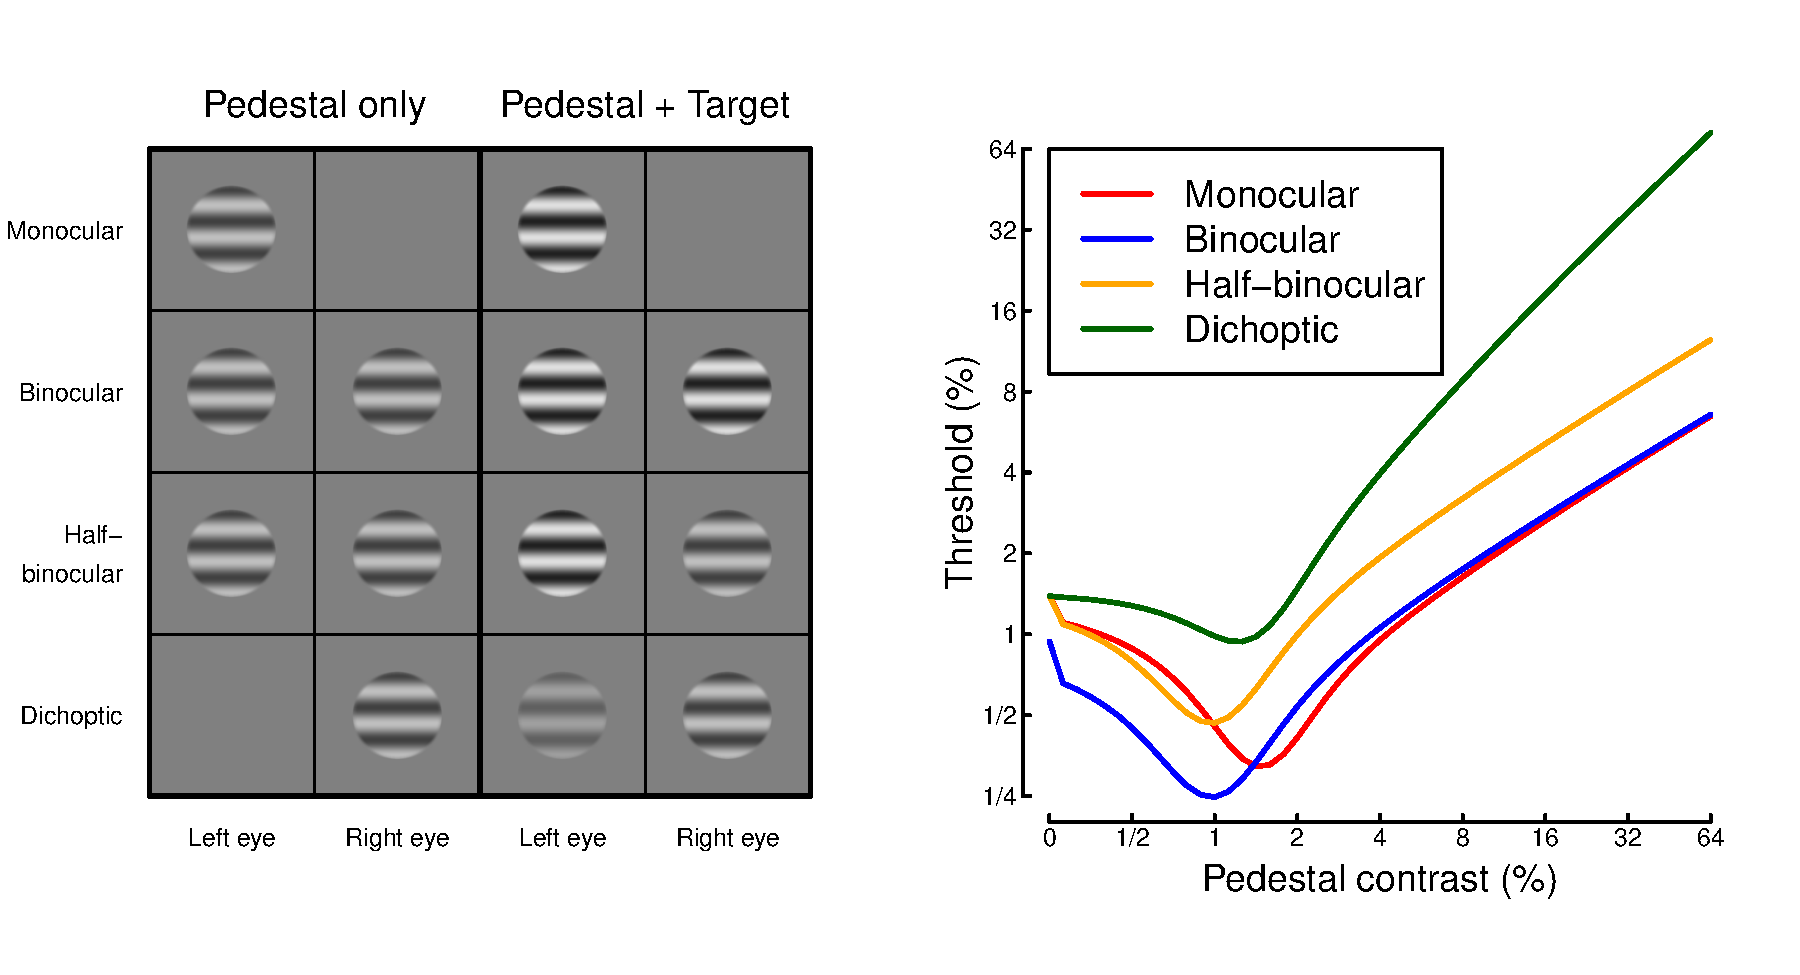
\includegraphics{Figures/exampledips.pdf}

}

\caption{\label{fig-exampledips}Illustration of stimulus conditions
(left) and example dipper functions (right).}

\end{figure}%

The detailed pattern of thresholds across these four conditions is
complex, and for achromatic stimuli has several distinctive features
that have been replicated in multiple studies. At low pedestal
contrasts, the binocular condition yields lower thresholds than the
monocular condition; this result is attributed to physiological
binocular summation by neurons responsive to signals from both eyes
(Baker et al., 2018; Campbell \& Green, 1965). However, at high pedestal
contrasts the `handle' regions of the dipper functions for these
conditions converge: a consequence of interocular suppression
compensating for the increased excitation during binocular stimulation
(Legge, 1984; Maehara \& Goryo, 2005). The half-binocular condition
avoids confounding the number of eyes seeing the target with the number
of eyes seeing the pedestal (Meese et al., 2006). The pedestal is always
binocular in this condition, whereas the target increment is monocular,
and thresholds are consistently higher than in the binocular condition
across the full range of pedestal contrasts. This demonstrates that
binocular summation occurs across the entire contrast range, when the
pedestal ocularity is appropriately controlled. Finally, the dichoptic
condition produces extremely strong masking of the target, such that
when the pedestal is visible, the target must equal or exceed its
contrast to be detectable (Baker \& Meese, 2007; Legge, 1979; Maehara \&
Goryo, 2005). The characteristic pattern of dipper functions (right
panel of Figure~\ref{fig-exampledips}) is well-described by the gain
control model of Meese et al. (2006) for achromatic stimuli.

At the output of the human retina, cone responses are split into three
distinct pathways. The sum of long- (L) and medium- (M) wavelength cone
outputs (L+M) transmits luminance information (see Sharpe et al., 2011),
and is likely responsible for the binocular combination effects
previously studied using achromatic stimuli (see above). The difference
of long- and medium-wavelength cone outputs (L-M) is responsive to
chromatic stimuli modulating along a red/green axis in colour space.
Finally the opponent short-wavelength (S) channel codes chromatic
stimuli modulating along a blue/yellow axis (S-(L+M)). At isoluminance,
where (L+M) is held constant, this channel is driven purely by the
S-cone outputs. Note that we use these shorthand terms throughout to
refer to chromatic mechanisms, but acknowledge that in reality the
photoreceptor outputs are weighted, for example S-0.5(L+M), and 3L+M.
Within each chromatic pathway, contrast discrimination functions (which
plot discrimination thresholds against pedestal contrast; sometimes
referred to as TvC functions) are similar to those for achromatic
vision, showing evidence of facilitation at low pedestal contrasts and
masking at high pedestal contrasts (Chen et al., 2000; Switkes et al.,
1988). There are also interactions between luminance and colour
mechanisms, which are able to mask each other (Chen et al., 2000; Mullen
\& Losada, 1994; Switkes et al., 1988), and under some circumstances
also show cross-pathway facilitation (Cole et al., 1990; Mullen \&
Losada, 1994; Shooner \& Mullen, 2020; Switkes et al., 1988).

There has not yet been a detailed investigation of binocular contrast
interactions in either chromatic pathway, however there are reasons to
believe they may differ from the achromatic pathway. At detection
threshold, binocular summation is greater for chromatic versus
achromatic stimuli (Simmons, 2005), implying a more linear initial stage
of processing. For cross-orientation masking, there are differences in
the magnitude of masking between chromatic (L-M) and achromatic stimuli
(Kim et al., 2013; Medina \& Mullen, 2009), as well as differences in
their temporal dynamics (Kim \& Mullen, 2015). There are also binocular
interactions between chromatic and achromatic pathways (Kingdom \&
Libenson, 2015; Mullen et al., 2014), yet these have not been fully
explored for arrangements where the target and mask have the same
orientation. Finally, the neurophysiological underpinnings of colour
vision may be distinct from those of the achromatic system. The
classical view was that in primary visual cortex (V1), chromatic signals
are processed in `blob' regions that are revealed by cytochrome oxidase
staining (Horton \& Hubel, 1981), and are largely monocular (Livingstone
\& Hubel, 1984). However subsequent work has revealed a large population
of colour-luminance neurons with a subset of colour-only ones, making
such a clear-cut physiological distinction unlikely (for a review, see
Shapley \& Hawken, 2011). Nevertheless, the physiological segregation
between pathways at the output of the retina could still lead to
differences in the way signals are combined across the eyes.

The spatiotemporal profile of stimuli also appears to impact their
binocular combination. For example, matching studies indicate that
binocular combination can be close to linear for luminance increments
(Anstis \& Ho, 1998; Levelt, 1965), particularly against a dark
background (Baker et al., 2012). This is quite different from the
`ocularity invariance' (where binocular and monocular stimuli appear
equal) that is well-established when using spatially modulated stimuli
such as sine-wave gratings, and implies strong interocular suppression
(Baker \& Wade, 2017; Meese et al., 2006; Moradi \& Heeger, 2009). Our
recent work (Segala et al., 2023) has investigated binocular combination
for flickering discs of luminance, which are DC-balanced across time
(i.e.~the time-averaged luminance is equal to the background).
Steady-state EEG responses from early visual cortex and psychophysical
contrast matching data were both consistent with weak interocular
suppression when using this stimulus arrangement, but it is currently
unclear whether this has implications for contrast discrimination
performance.

The main aim of the present study was to characterise binocular signal
combination for chromatic stimuli, and for temporal modulations of
luminance. We also aimed to investigate interocular suppression between
chromatic and achromatic pathways. We therefore preregistered a series
of psychophysical experiments (see: \url{https://osf.io/3vdga/}). In
Experiment 1 we replicate the four key pedestal masking conditions of
Meese et al. (2006) described above for achromatic grating stimuli and
extend this to both L-M and S-(L+M) isoluminant chromatic stimuli. In
Experiment 2 we explore dichoptic masking within and between these
stimuli. Experiment 3 repeats the achromatic condition from the first
experiment but using a temporally modulated disc rather than sine-wave
gratings. We take a Bayesian approach to data analysis and modelling; by
fitting a hierarchical version of the two-stage gain control model
(Meese et al., 2006) we compare posterior parameter distributions to
understand how model parameters such as the weight of interocular
suppression vary across visual pathways.

\section{Materials \& Methods}\label{materials-methods}

\subsection{Participants}\label{participants}

All experiments were completed by the first author (DHB) and two
additional participants, who differed for each experiment. Participants
had no known abnormalities of binocular or colour vision. Written
informed consent was obtained before data collection began, and all
procedures were approved by the ethics committee of the Department of
Psychology at the University of York (ID number 2202). The study
conformed to the tenets of the Declaration of Helsinki.

\subsection{Apparatus \& stimuli}\label{apparatus-stimuli}

In Experiments 1 and 2, the stimuli were horizontal sinusoidal gratings
with a spatial frequency of 1c/deg (see examples in
Figure~\ref{fig-examplestim}). The gratings were windowed by a raised
cosine envelope with a diameter of 3 degrees. Spatial phase, relative to
a central fixation cross, was randomised on each trial across the four
cardinal phases. In the achromatic conditions, the sine-wave modulated
all three monitor colour channels equally (red, green and blue). In the
L-M condition, we generated isoluminant stimuli for each participant
(see Procedures) designed to maximise contrast between L and M cones,
whilst keeping S cone activity constant (more accurately, this is a
\(\Delta L/L - \Delta M/M\) condition, see Cole et al., 1993). In the
S-(L+M) condition (or more accurately the
\(\Delta S/S - (\Delta L/L + \Delta M/M)\) condition), the isoluminant
stimuli maximised S-cone contrast. Stimuli were converted from cone
space to monitor RGB coordinates using the monitor spectral readings and
the Stockman-Sharpe 2 degree cone fundamentals (Stockman \& Sharpe,
2000). The maximum displayable cone contrasts on our system were 0.1 for
L-M, and 0.88 for S-(L+M). The stimuli in Experiment 3 were temporal
modulations of luminance applied to a disc made using the same raised
cosine envelope as described above, but with no further spatial
modulation. The stimuli counterphase flickered sinusoidally at 4Hz (see
examples in the lower portion of Figure~\ref{fig-examplestim}). In all
experiments, we displayed a binocular fusion lock, consisting of three
concentric rings of small square elements with random colour. A black
central fixation cross was also displayed throughout.

\begin{figure}

\centering{

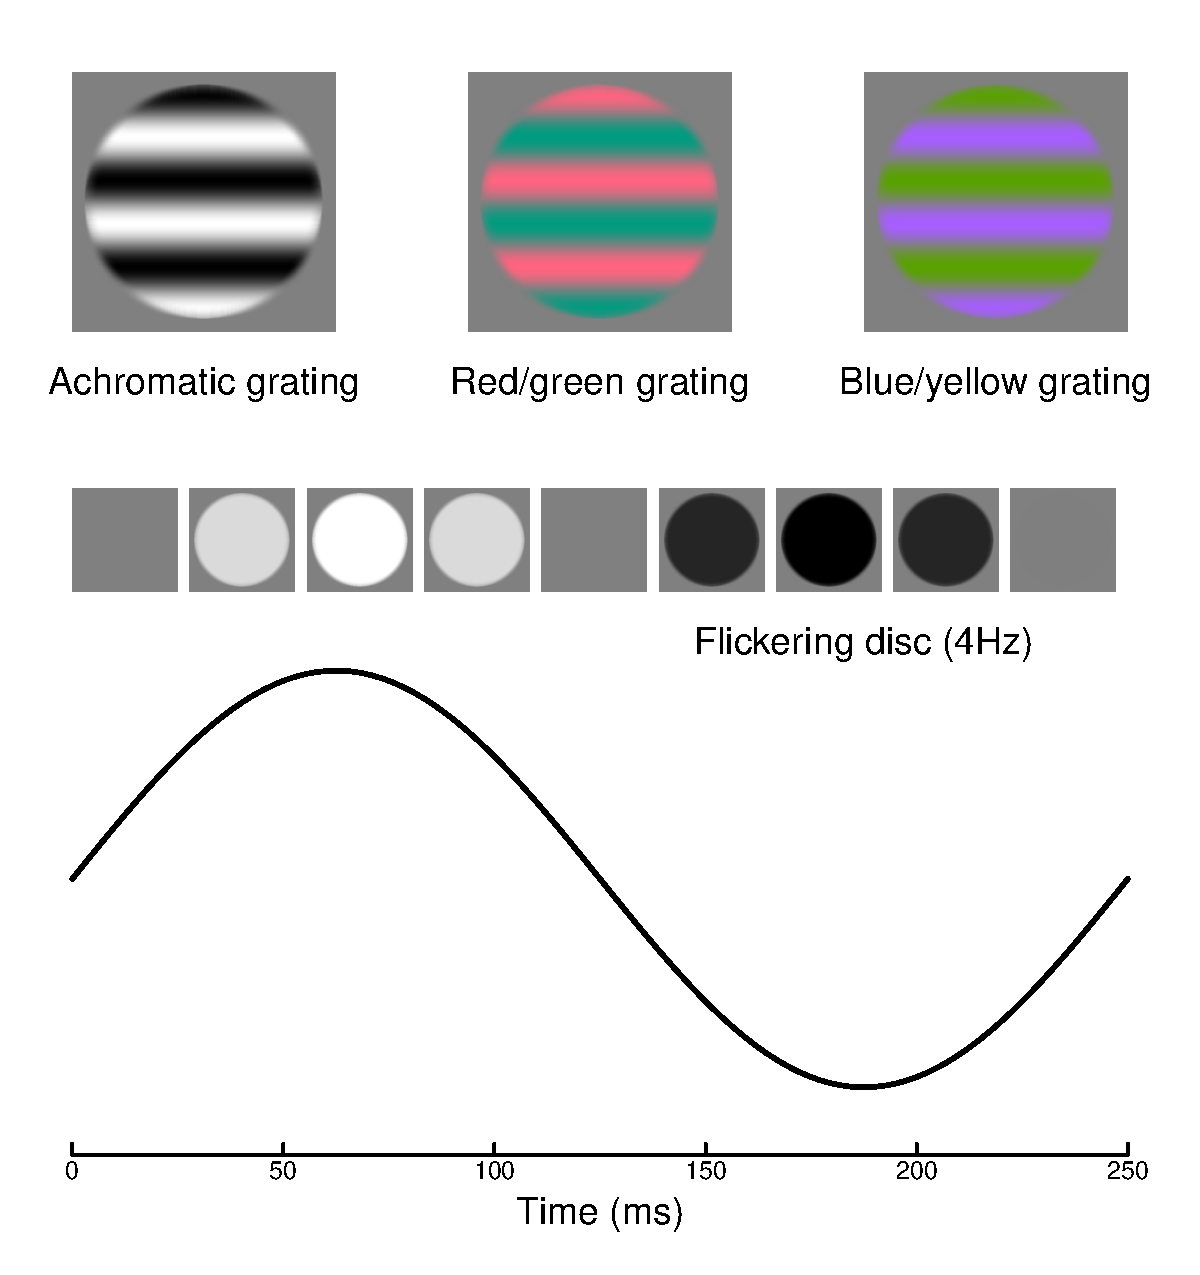
\includegraphics[width=0.5\textwidth,height=\textheight]{Figures/examplestim.pdf}

}

\caption{\label{fig-examplestim}Example stimuli. Upper row shows grating
stimuli used in Experiments 1 and 2. Lower row shows one cycle of
sinusoidal flicker applied to a uniform disc. Note that the rendering of
all stimuli will depend on the device used to display or print this
image, and so the chromatic stimuli are unlikely to appear isoluminant,
and there may be additional luminance nonlinearities that were not
present in the stimuli displayed during the experiments.}

\end{figure}%

All stimuli were presented on an Iiyama VisionMaster Pro 510 CRT
monitor, with a refresh rate of 100Hz, and a resolution of 1024 x 768
pixels. The display was driven by a ViSaGe MkII stimulus generator
(Cambridge Research Systems Ltd., Kent, UK) running in 42-bit colour
mode (14 bits per colour channel). We presented stimuli to the left and
right eyes independently using a four-mirror stereoscope with
front-silvered mirrors. The display was luminance calibrated using a
ColourCal photometer (Cambridge Research Systems), and gamma corrected
by fitting a four-parameter gamma function to the output of each CRT
gun. The maximum luminance was 87 cd/m\(^2\). We also measured the
spectral output of each phosphor using a Jaz spectroradiometer (Ocean
Insight, Florida), and used these measurements to convert between LMS
(cone) space and the monitor RGB coordinates. We express threshold and
pedestal contrasts in normalized units, relative to the monocular
detection threshold for each stimulus type. A threshold value of 2
therefore means that, relative to monocular detection, twice as much
contrast was required to reach the same level of performance.

\subsection{Procedure}\label{procedure}

All experiments took place in a darkened room. Participants placed their
heads in a chin rest mounted on a height-adjustable table, to which the
stereoscope was also attached. The total optical viewing distance
(including the light path through the mirrors) was 104cm, at which
distance 1 degree of visual angle encompassed 48 pixels on the monitor.

Before beginning primary data collection, each participant in
Experiments 1 and 2 completed an isoluminance adjustment task. Grating
stimuli were presented that counterphase flickered at 5Hz, with contrast
variations defined about either the L-M or S-(L+M) plane in cone space.
Participants used a trackball to dynamically adjust the colour angle of
the stimulus to minimise the percept of flicker. Each participant
completed ten such trials for each colour plane, and the average angle
across repetition was taken as the isoluminant point, and used to
generate stimuli in the main experiment for that participant. Settings
were very similar across participants for the S-(L+M) direction, and
somewhat more heterogeneous for the L-M direction (see
Figure~\ref{fig-isofig}).

\begin{figure}

\centering{

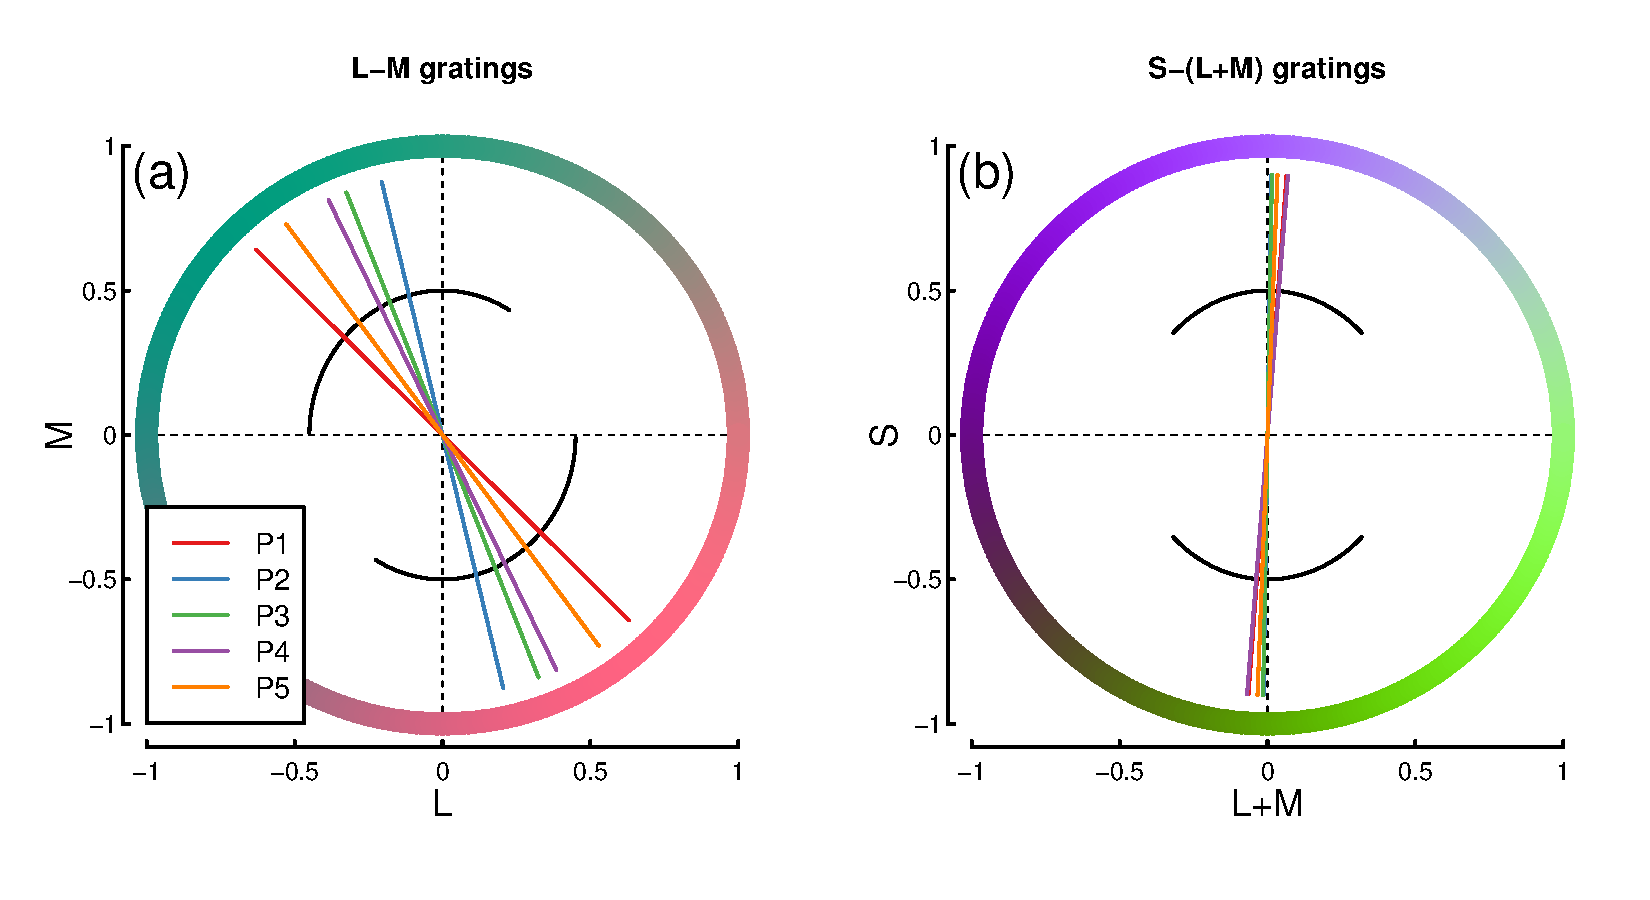
\includegraphics{Figures/isosettings.pdf}

}

\caption{\label{fig-isofig}Isoluminance settings from all participants
in Experiments 1 and 2. Panel (a) shows L-M and panel (b) shows S-(L+M)
settings that were subsequently used to generate stimuli in the main
experiments. Within each panel, solid lines show the mean settings for
each participant, and black curves show the range of possible stimuli
displayed during the adjustment task.}

\end{figure}%

In Experiment 1, participants completed a two-interval-forced-choice
(2IFC) contrast discrimination task. Stimuli were presented for 200ms,
with an interstimulus interval of 400ms. Each interval was indicated by
an auditory beep, and participants made their responses using a
two-button trackball. Correct responses were followed by a high-pitched
tone, and incorrect responses by a low-pitched tone. Each block of the
experiment tested a single pedestal contrast level and lasted around 12
minutes. The pedestal contrasts were 0, 0.5, 1, 2, 4, 8, 16 and 32\%
Michelson contrast for the achromatic stimulus, and 0, 1, 2, 4, 8, 16,
32 and 64\% of the maximum available contrast for each chromatic
stimulus. On each trial the target contrast level was determined by a
3-down-1-up staircase procedure, moving in logarithmic (3dB) steps.
There were 8 interleaved staircases in total; four stimulus arrangements
(see Figure~\ref{fig-exampledips}) combined factorially with two target
eye assignments. Each pedestal contrast was repeated 3 times by each
participant, and the block order was randomised. The experiment lasted
around 4 hours per participant for each chromatic condition, and took
place over the course of several weeks. In total, the experiment
consisted of 67978 trials (pooled across participants).

In Experiment 2, participants completed a 2IFC dichoptic masking task.
The stimuli and trial protocol were the same as for Experiment 1, except
that the target contrast was chosen from a set of 10 possible values,
determined in advance based on the data of Experiment 1. There were 12
possible conditions: baseline detection thresholds for achromatic, L-M
and S-(L+M) stimuli, and the nine possible factorial pairings obtained
by assigning these conditions to be target and dichoptic mask stimuli.
Mask contrasts were chosen to be approximately 16 times their
(monocular) detection threshold, based on the data from Experiment 1.
The contrasts were 16\% Michelson contrast for the achromatic stimuli,
6.4\% cone contrast for L-M and 56\% cone contrast for S-(L+M). Each
block of the experiment tested a single condition, and consisted of 200
trials. A high contrast example of the target stimulus was displayed at
the foot of the screen throughout, so that there was no ambiguity about
the target identity on a given block. Participants completed 10
repetitions of each condition (120 blocks of \textasciitilde6 minutes
each), lasting around 12 hours, for a total of 72000 trials (pooled
across participants).

In Experiment 3, the achromatic conditions from Experiment 1 were
repeated using a flickering disc stimulus. The stimulus counterphase
flickered at 4Hz, and was presented for 500ms (i.e.~2 full cycles of the
temporal modulation). All other procedures were the same as for
Experiment 1, and the experiment comprised a total of 24610 trials
(pooled across participants).

\subsection{Data analysis and computational
modelling}\label{data-analysis-and-computational-modelling}

Psychometric functions from each experiment were fit using
\emph{psignifit} 4 to estimate threshold and slope parameters via a
Bayesian numerical integration method (Schütt et al., 2016). A
cumulative Gaussian was used as the underlying function, with contrast
values expressed in decibel (dB) units (where
\(C_{dB} = 20log_{10}(C_\%)\)). We converted the slope estimates
(\(\sigma\) parameters from the fitted Gaussians) to equivalent Weibull
\(\beta\) values using the approximation \(\beta = 10.3/\sigma\).
Threshold was defined as the target contrast corresponding to an
accuracy of 75\% correct.

The two-stage model of Meese et al. (2006) was fit to the threshold data
from Experiments 1 and 3 using a simplex algorithm to minimise the error
between the model and data. We normalized the thresholds and pedestal
contrasts to the appropriate monocular threshold for each stimulus type.
The model is defined by a series of equations:

\begin{equation}\phantomsection\label{eq-s1l}{\mathrm{Stage1}_L = \frac{C_L^m}{S + C_L + \omega C_R},}\end{equation}

\begin{equation}\phantomsection\label{eq-s1r}{\mathrm{Stage1}_R = \frac{C_R^m}{S + C_R + \omega C_L},}\end{equation}

\begin{equation}\phantomsection\label{eq-binsum}{\mathrm{binsum} = \mathrm{Stage1}_L + \mathrm{Stage1}_R,}\end{equation}

\begin{equation}\phantomsection\label{eq-s2}{\mathrm{Stage2} = \frac{\mathrm{binsum}^p}{Z + \mathrm{binsum}^q},}\end{equation}

where \(C_L\) and \(C_R\) are the (normalized) contrasts displayed to
the left and right eyes, and \(m\), \(S\), \(\omega\), \(p\), \(q\) and
\(Z\) are free parameters in the model. A further free parameter, \(k\),
is used to convert the model outputs to either d-prime or threshold
values (note that in the original model specification (Meese et al.,
2006) this parameter was called \(\sigma\), but we use the \(k\) symbol
here to avoid confusion with the standard deviation of the cumulative
Gaussian used when fitting the psychometric functions to estimate
thresholds). Thresholds are defined by iteratively adjusting the target
contrast until the following equality is satisfied:

\begin{equation}\phantomsection\label{eq-thd}{\mathrm{Stage2}_{\mathrm{target+pedestal}} - \mathrm{Stage2}_{\mathrm{pedestal}} = k,}\end{equation}

and \(d'\) (d-prime) for a single target level is defined as:

\begin{equation}\phantomsection\label{eq-dprime}{d' = \frac{\mathrm{Stage2}_{\mathrm{target+pedestal}} - \mathrm{Stage2}_{\mathrm{pedestal}}}{k/\tau},}\end{equation}

where the parameter \(\tau\) reflects the value of \(d'\) at detection
threshold. Defining threshold as the 75\% correct point on the
psychometric function (as here) yields a value of
\(\tau = \Phi^{-1}(0.75)\sqrt{2}\) = 0.954 (where \(\Phi^{-1}\) is the
inverse cumulative normal density function). The combined denominator
term (\(k/\tau\)) therefore represents internal additive noise in the
model.

We ran the simplex algorithm from 100 random starting vectors for each
data set, and chose the solution for each data set that gave the
smallest root mean squared error (RMSE) between the model and data.

We also implemented a Bayesian hierarchical version of the model using
the Stan probabilistic programming language (Carpenter et al., 2017).
This used a binomial generator function to model the proportion correct
data at each target level, and was fit simultaneously to all
participants for a given experiment, but separately for each chromatic
condition of Experiment 1, and the flickering disc data from Experiment
3 (i.e.~four fits in total, as for the simplex fitting). Prior
distributions for the parameters \emph{p}, \emph{q}, \emph{m} and
\(\omega\) were Gaussian, with means determined from published values
(see first row of Table~\ref{tbl-parametertable}). Priors for parameters
\emph{S}, \emph{Z} and \emph{k} were uniform. This modelling primarily
focuses on examining posterior parameter distributions, rather than a
model comparison approach. We generated over 1 million posterior samples
for the model, and retained 10\% of them for plotting.

Finally, we adapted the two stage model to include parallel pathways to
process achromatic, L-M and S-(L+M) stimuli, that mutually suppress each
other. We added additional suppressive terms at the first (monocular)
stage of the model, for example:

\begin{equation}\phantomsection\label{eq-s1multi}{^{AC}\mathrm{Stage1}_L = \frac{AC_L^m}{S + AC_L + \omega_A AC_R + \omega_R RG_R + \omega_B BY_R},}\end{equation}

where \emph{AC} represents the achromatic contrast, \emph{RG} represents
the L-M contrast, \emph{BY} represents the S-(L+M) contrast, and
\(\omega_A\), \(\omega_R\) and \(\omega_B\) are the accompanying weights
of interocular suppression. There is an equivalent expression for the
right eye, and for each of the two isoluminant chromatic pathways. To
simplify the model, and avoid free parameters that are poorly
constrained by the data, we fixed several parameters (\emph{p},
\emph{q}, \emph{m}, \emph{S}, \emph{k}, and \(\omega\) for the
within-pathway suppression) at the values from the fits from Experiment
1 (Table~\ref{tbl-parametertable}, lower rows). This left 9 free
parameters: a \(Z\) parameter for each mechanism, and six
cross-mechanism weights of interocular suppression. These parameters
were again estimated within a Bayesian hierarchical framework, using the
binomial proportion correct data from Experiment 2. Note that the model
as specified does not currently include monocular suppression between
different pathways, as we did not collect any data for these conditions.
Previous work (e.g. Chen et al., 2000; Mullen \& Losada, 1994) has
measured such interactions, and they could in principle be incorporated
into the denominator of either stage 1 or stage 2 in the model.

\subsection{Open science practices}\label{open-science-practices}

All experimental code, raw data and analysis scripts are available at:
https://osf.io/3vdga/. The linked GitHub repository also contains a
fully computationally reproducible version of the manuscript. Note that
we deviated slightly from the planned preregistration, in that we did
not collect data for chromatic flickering discs, or for the
cross-pathway dichoptic experiment using disc stimuli. This is because
the grating data from Experiments 1 and 2, and the achromatic disc data
from Experiment 3, were sufficient to address the questions we had hoped
to answer from these experiments.

\section{Results}\label{results}

\subsection{Experiment 1}\label{experiment-1}

Dipper functions from Experiment 1 are displayed in the upper row of
Figure~\ref{fig-dipperfig}. Panel (a) shows the achromatic results,
which replicate the key features from previous work. At detection
threshold, binocular summation was a factor of 1.67 (4.47dB), within the
range (\(\sqrt{2}\) to 2) consistent with previous reports (Baker et
al., 2018). Pedestal masking functions followed the typical `dipper'
shape in all conditions, with a region of facilitation at low pedestal
contrasts, and masking at higher contrasts. The monocular and binocular
dipper handles converge at high contrasts, whereas the half-binocular
thresholds remain above the binocular thresholds across the full range
of pedestal contrasts. The dichoptic condition produced very high
thresholds, with the rising portion of the dipper having a slope around
1 (regression slope of 1.06 in log (dB) units, calculated across the
highest 4 pedestal contrasts).

\begin{figure}

\centering{

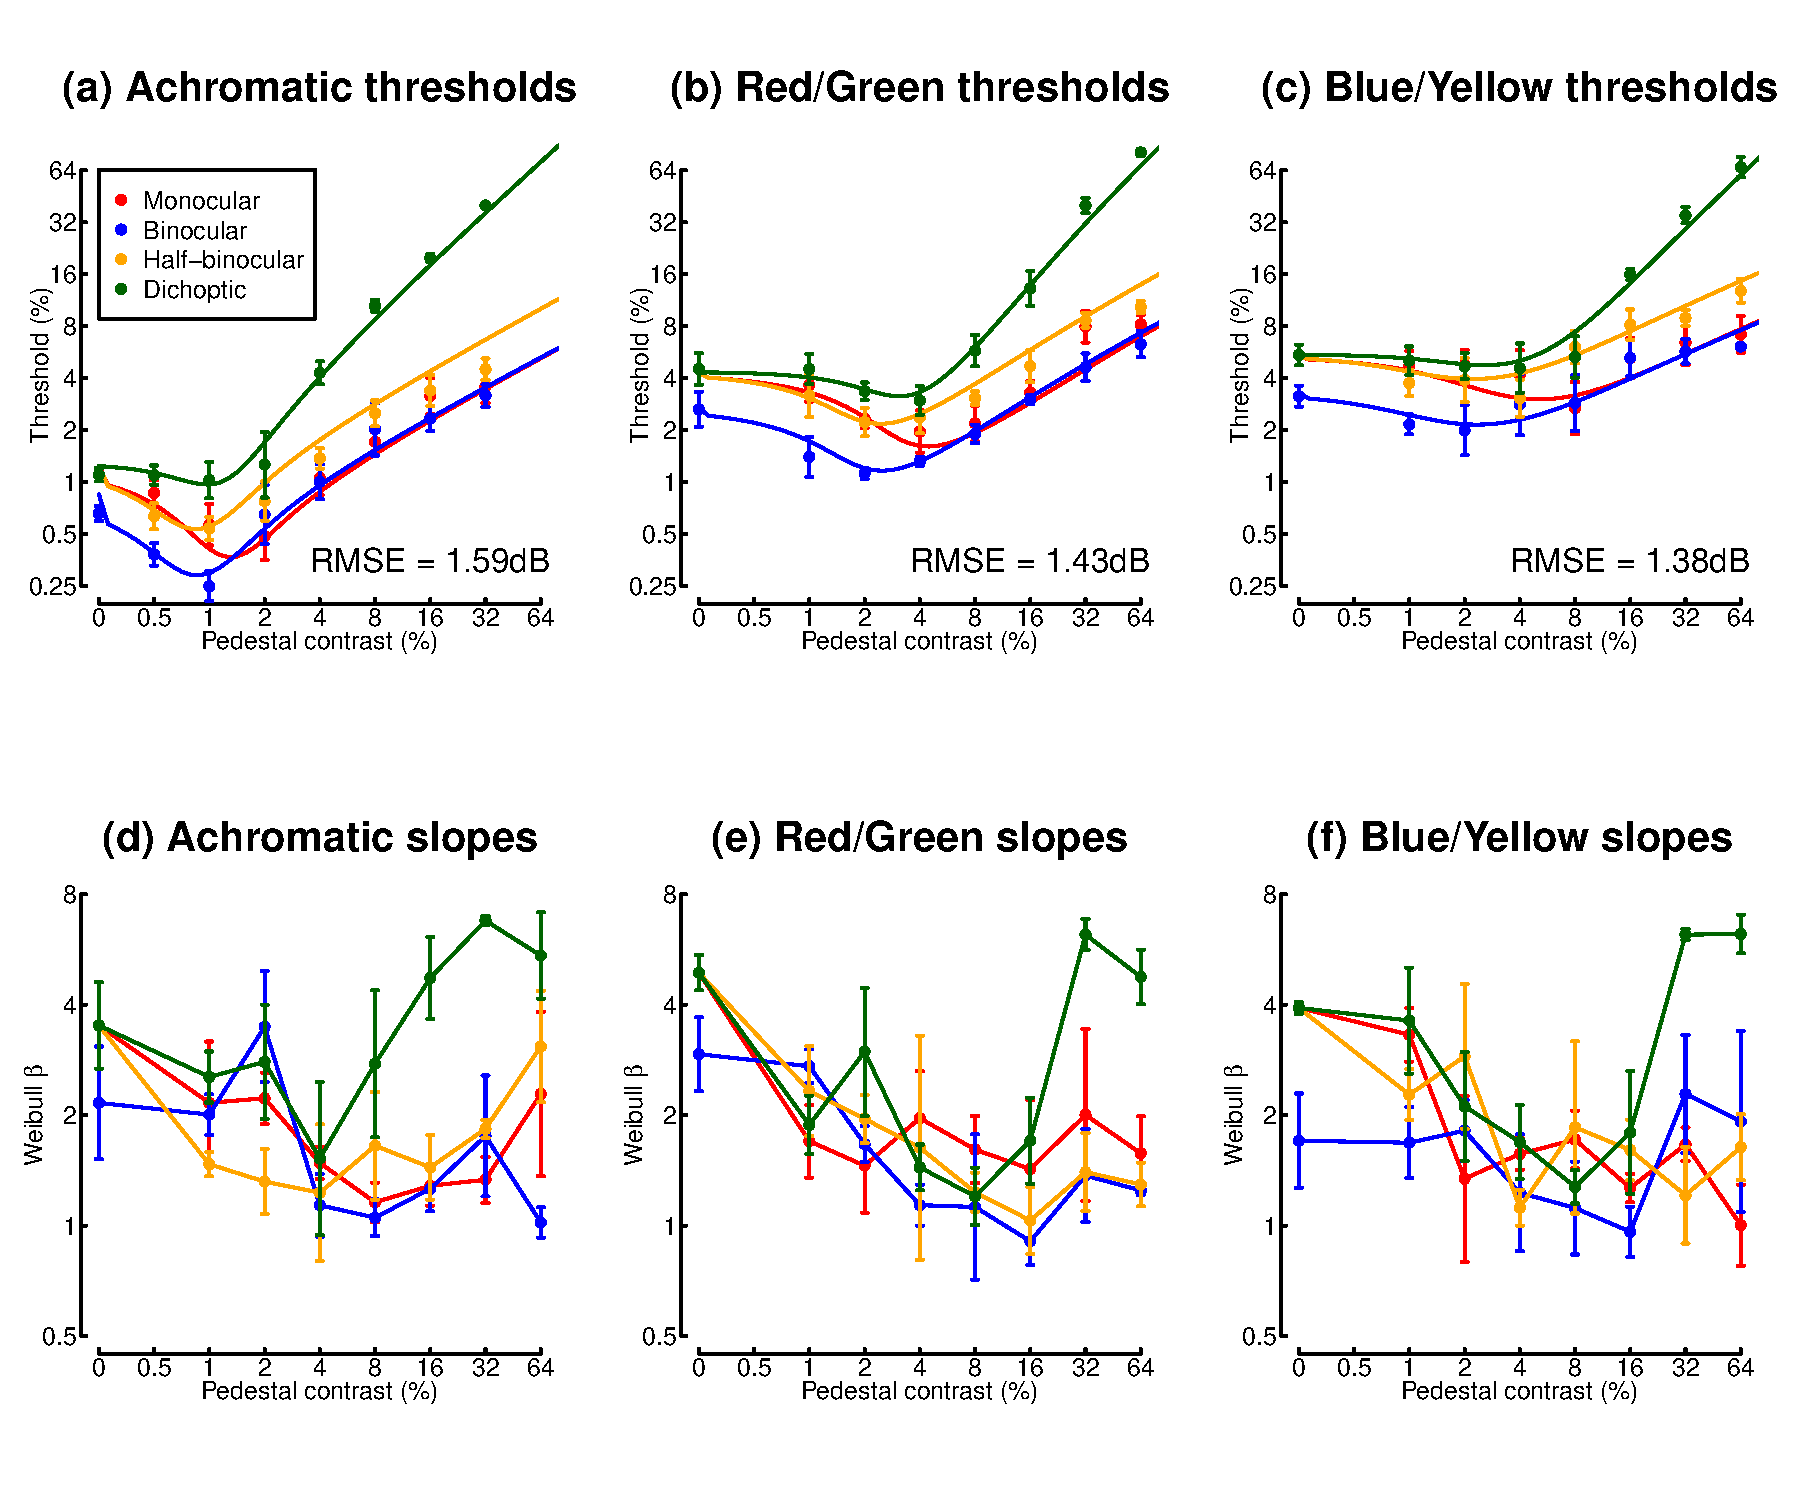
\includegraphics{Figures/dipperssimplex.pdf}

}

\caption{\label{fig-dipperfig}Dipper functions and psychometric slopes
from Experiment 1, averaged across three participants. Panels (a-c) show
threshold data, and panels (d-f) represent the slope of the psychometric
function expressed in Weibull \(\beta\) units. Error bars give ±1SE
across participants. Note that all contrast values for both thresholds
and pedestals are normalized to the monocular detection threshold in
each panel. Curves in panels (a-c) show the best fitting models,
optimized using a simplex algorithm, and RMSE values give the root mean
squared errors of the fits.}

\end{figure}%

A similar pattern of results was observed for both the L-M and S-(L+M)
isoluminant stimuli (see Figure~\ref{fig-dipperfig}b,c). Summation at
threshold was a factor of 1.71 (4.66dB) for the L-M targets, and a
factor of 1.73 (4.77dB) for the S-(L+M) targets, and so was marginally
higher than for achromatic stimuli. The general character of the dipper
functions was largely consistent with the achromatic results, though we
observed shallower facilitation and weaker masking, especially for the
S-(L+M) stimuli. For example, the strongest facilitation in the
binocular condition for achromatic stimuli was a factor of 2.63, whereas
it reduced to a factor of 2.35 for L-M stimuli and 1.57 for S-(L+M)
stimuli. The slope of the binocular dipper handle was 0.52 for
achromatic stimuli, 0.58 for L-M stimuli, and 0.34 for S-(L+M) stimuli.
Dichoptic masking remained as strong for the chromatic conditions as for
the achromatic stimuli (regression slopes of 1.3 for L-M and 1.21 for
S-(L+M)). The pattern of results for individual participants was
consistent with the group averages, as shown in
Figure~\ref{fig-individualdippers}.

Following Meese et al. (2006), we also inspected the slope of the
psychometric function for each condition (see
Figure~\ref{fig-dipperfig}d-f), as this provides information about the
effective gradient of the underlying contrast response function. At
detection threshold, slopes were relatively steep for all stimuli, with
values around \(\beta=4\). As pedestal contrasts increased, slopes
linearized and reduced to around \(\beta=1.3\) (Foley \& Legge, 1981;
Meese et al., 2006), and remained shallow at high pedestal contrasts.
The exception to this was the dichoptic condition, where slopes became
extremely steep at high dichoptic mask contrasts, consistent with
previous observations (Baker et al., 2013; Meese et al., 2006). This was
clear for all three data sets, with slope values in the range
\(4 < \beta < 8\). However, we observe that slope estimates are more
variable than threshold estimates (note the large error bars),
particularly when using adaptive staircases, which deploy most trials
close to threshold. Our second experiment therefore investigated the
slope of the psychometric function in more detail for dichoptic masking
using the method of constant stimuli, as well as exploring dichoptic
interactions between chromatic channels.

\subsection{Experiment 2}\label{experiment-2}

In Experiment 2 we focussed on the dichoptic condition at a single mask
contrast, and measured full psychometric functions using the method of
constant stimuli for all factorial pairings of target and mask
chromaticity. The pooled results across three participants are shown in
Figure~\ref{fig-MCSfig}a-c, and results for individual participants are
available in Figure~\ref{fig-individualMCS}. All conditions produced
monotonically increasing psychometric functions (panels a-c), but the
extent of masking was highly dependent on the relationship between the
target and mask chromaticity. Figure~\ref{fig-MCSfig}d-f shows a
two-dimensional representation of individual threshold and slope
estimates (points), as well as the posterior density estimates for fits
to the pooled data (ellipses). The results are consistent between
participants, and at the group level, and show that the presence of a
mask has a strong effect on thresholds.

\begin{figure}

\centering{

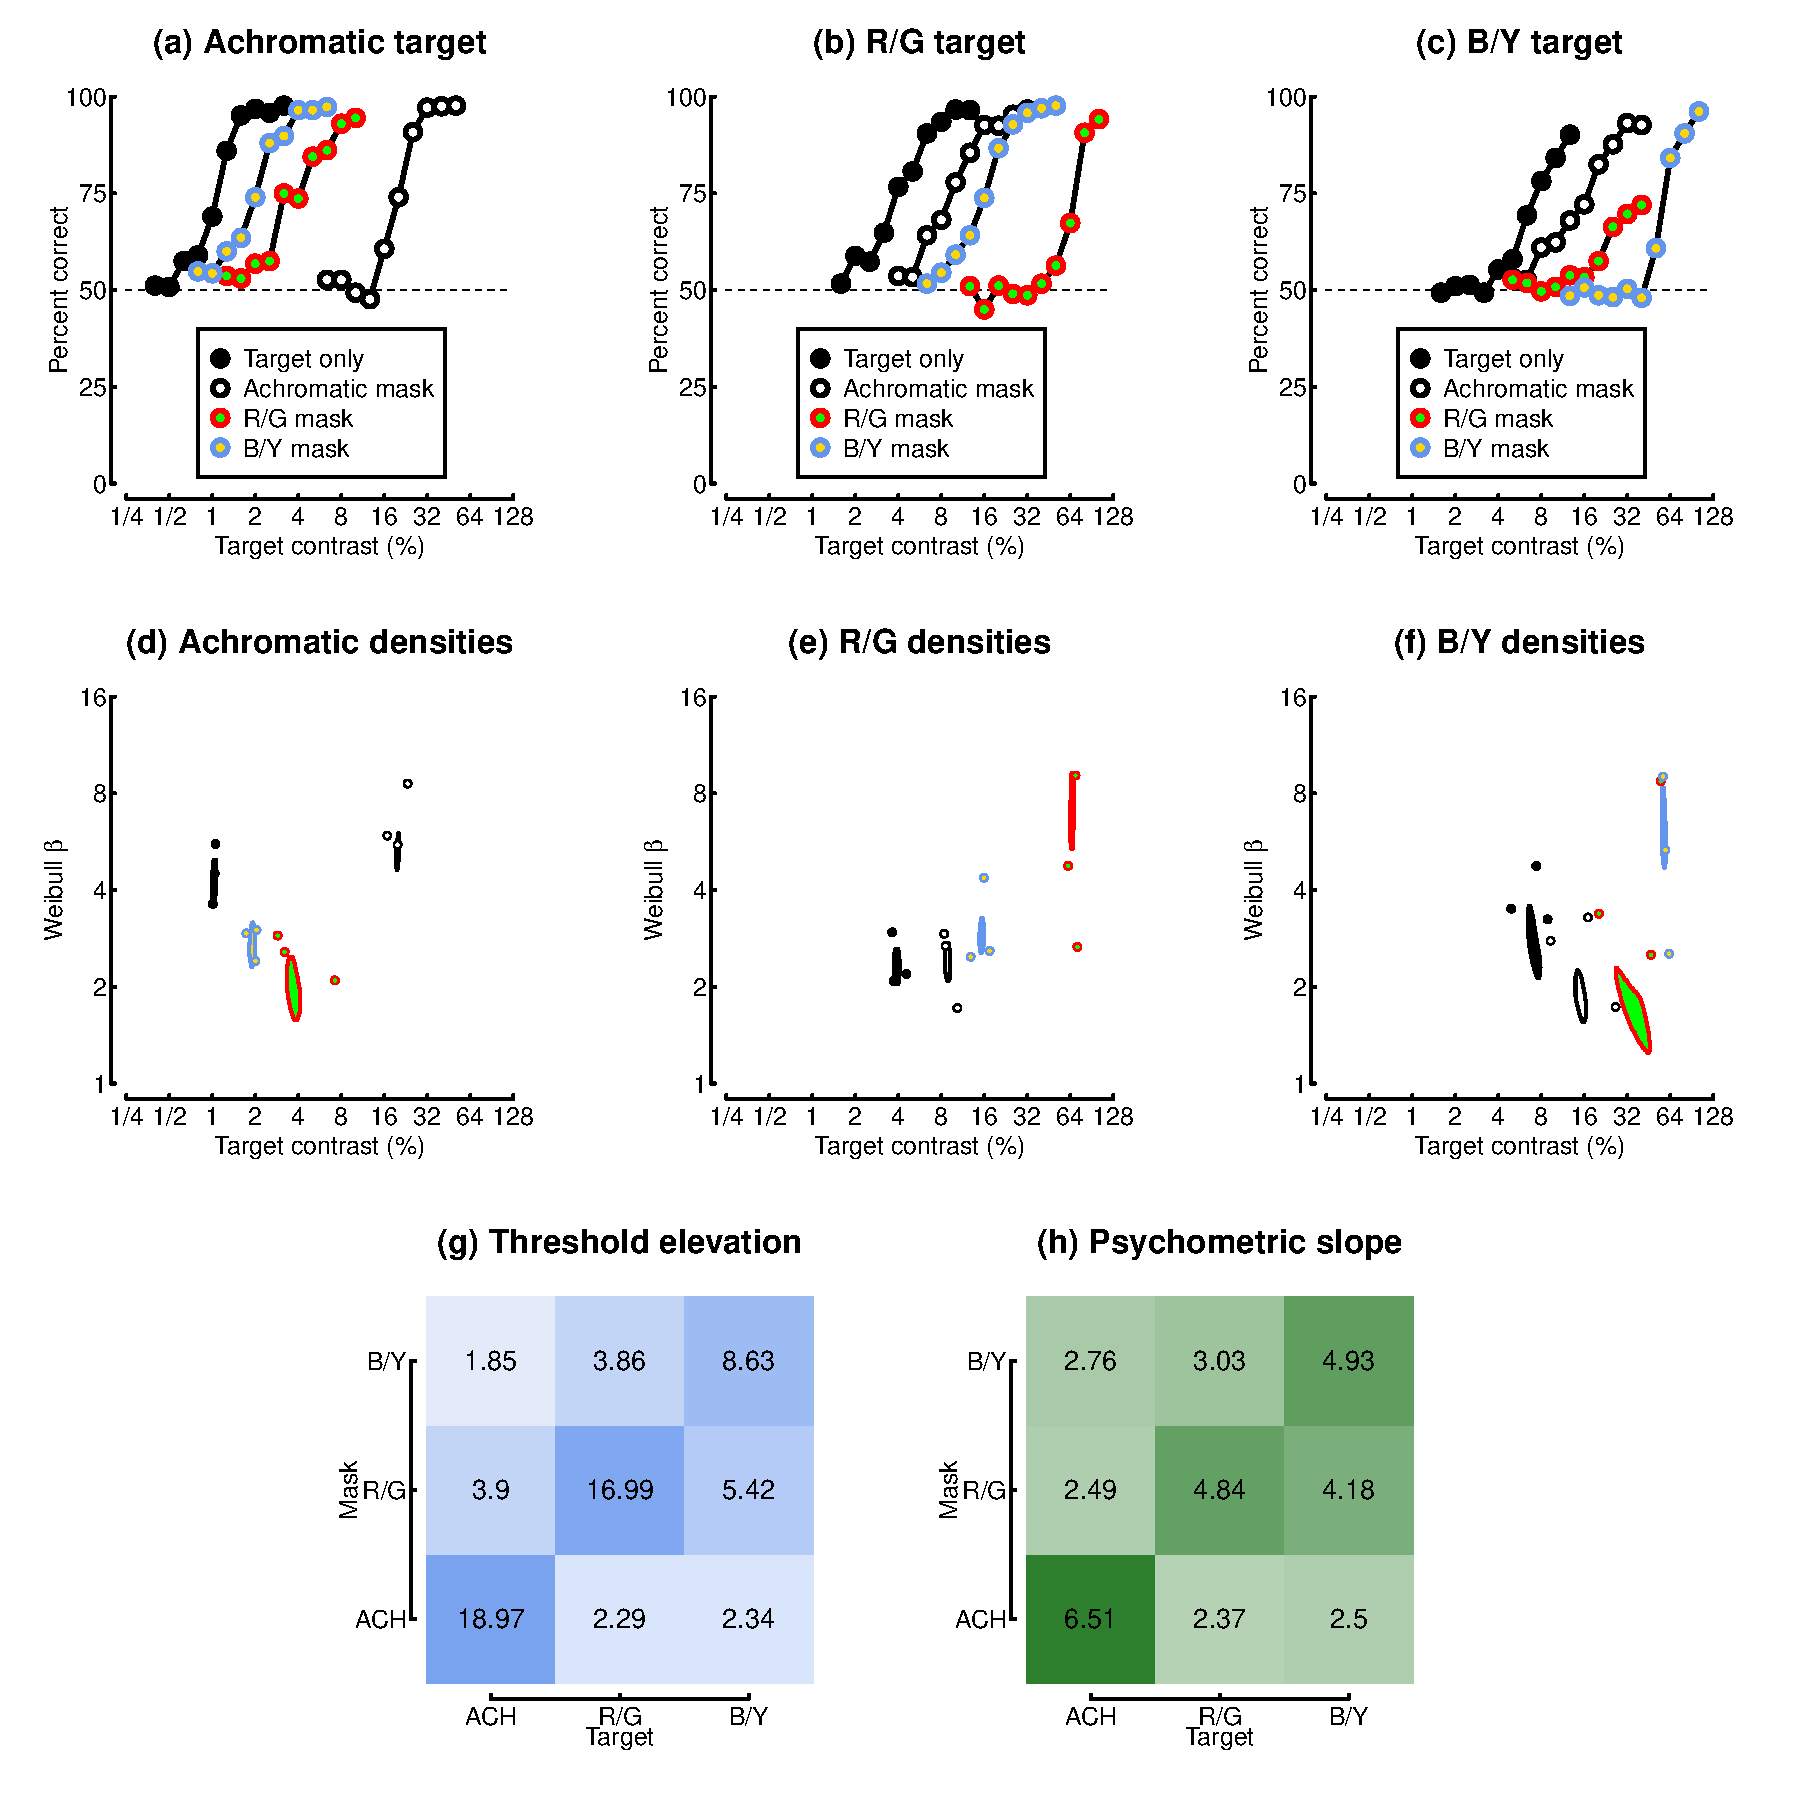
\includegraphics{Figures/MCSdata.pdf}

}

\caption{\label{fig-MCSfig}Summary of data from Experiment 2. Panels
(a-c) show psychometric functions for each condition, pooled across
participants (600 trials per target contrast level). Panels (d-f) show
threshold and slope estimates for individual participants (points) and
the boundary of the posterior density estimates for fits to the pooled
data (ellipses). Panel (g) shows the average threshold elevation factor
for each combination of target and mask stimulus. Panel (h) shows the
geometric mean psychometric slope value for each masking condition,
expressed in Weibull \(\beta\) units. Contrast values are normalized to
the target only threshold for each stimulus type.}

\end{figure}%

Threshold elevation was greatest when the target and mask had the same
chromaticity - notice that the psychometric function is shifted furthest
to the right for the achromatic target with an achromatic mask (white
and black circles in Figure~\ref{fig-MCSfig}a), for the L-M target with
an L-M mask (red and green circles in Figure~\ref{fig-MCSfig}b), and for
the S-(L+M) target with a S-(L+M) mask (blue and yellow circles in
Figure~\ref{fig-MCSfig}c). Masking was weakest between achromatic
masks/targets and chromatic masks/targets. Finally, there was an
intermediate level of masking between L-M and S-(L+M) stimuli. This is
summarised in Figure~\ref{fig-MCSfig}g, which represents threshold
elevation for each combination of target and mask chromaticity. Note
that the positive diagonal exhibits the highest values, and represents
threshold elevation between targets and masks of the same chromaticity.

We also calculated the slope of the psychometric function for each
condition, in equivalent Weibull \(\beta\) units. In the absence of a
mask, the average slope was \(\beta\) = 3.42, which is typical for
contrast detection tasks (Wallis et al., 2013). Slopes became
substantially steeper when the dichoptic mask matched the target in
chromaticity (average \(\beta\) = 5.38). These `super-steep'
psychometric functions for dichoptic pedestal masking have been reported
previously (Baker et al., 2013; Meese et al., 2006), and are observed
for the first time here using chromatic stimuli (see diagonal values in
Figure~\ref{fig-MCSfig}h, and also Figure~\ref{fig-dipperfig}d-f).
However, we did not see such markedly steep functions for any of the
cross-chromaticity masking conditions (average \(\beta\) = 2.83 for the
off-diagonal values).

\subsection{Experiment 3}\label{experiment-3}

In our final experiment, we again measured dipper functions, but this
time for a disc temporally modulating in luminance. This was motivated
by our recent work (Segala et al., 2023) that appeared to show increased
binocular facilitation and reduced interocular suppression for
flickering disc stimuli (relative to gratings), measured using EEG and a
psychophysical matching paradigm. The pattern of dipper functions for a
4Hz flickering disc (see Figure~\ref{fig-discdata}a) was very similar to
that observed for achromatic gratings (see Figure~\ref{fig-dipperfig}a),
and the binocular summation ratio at threshold was also similar (a
factor of 1.49 for discs, vs 1.67 for gratings). Threshold data for
individual participants are shown in Figure~\ref{fig-individualdiscs}.
We also found a similar pattern of psychometric slope values
(Figure~\ref{fig-discdata}b) as we had for gratings, though we note that
the dichoptic condition did not produce the `super-steep' psychometric
functions we had observed in Experiments 1 \& 2. Nevertheless, the
dichoptic slopes are somewhat above those of the other pedestal
arrangements at high contrasts.

\begin{figure}

\centering{

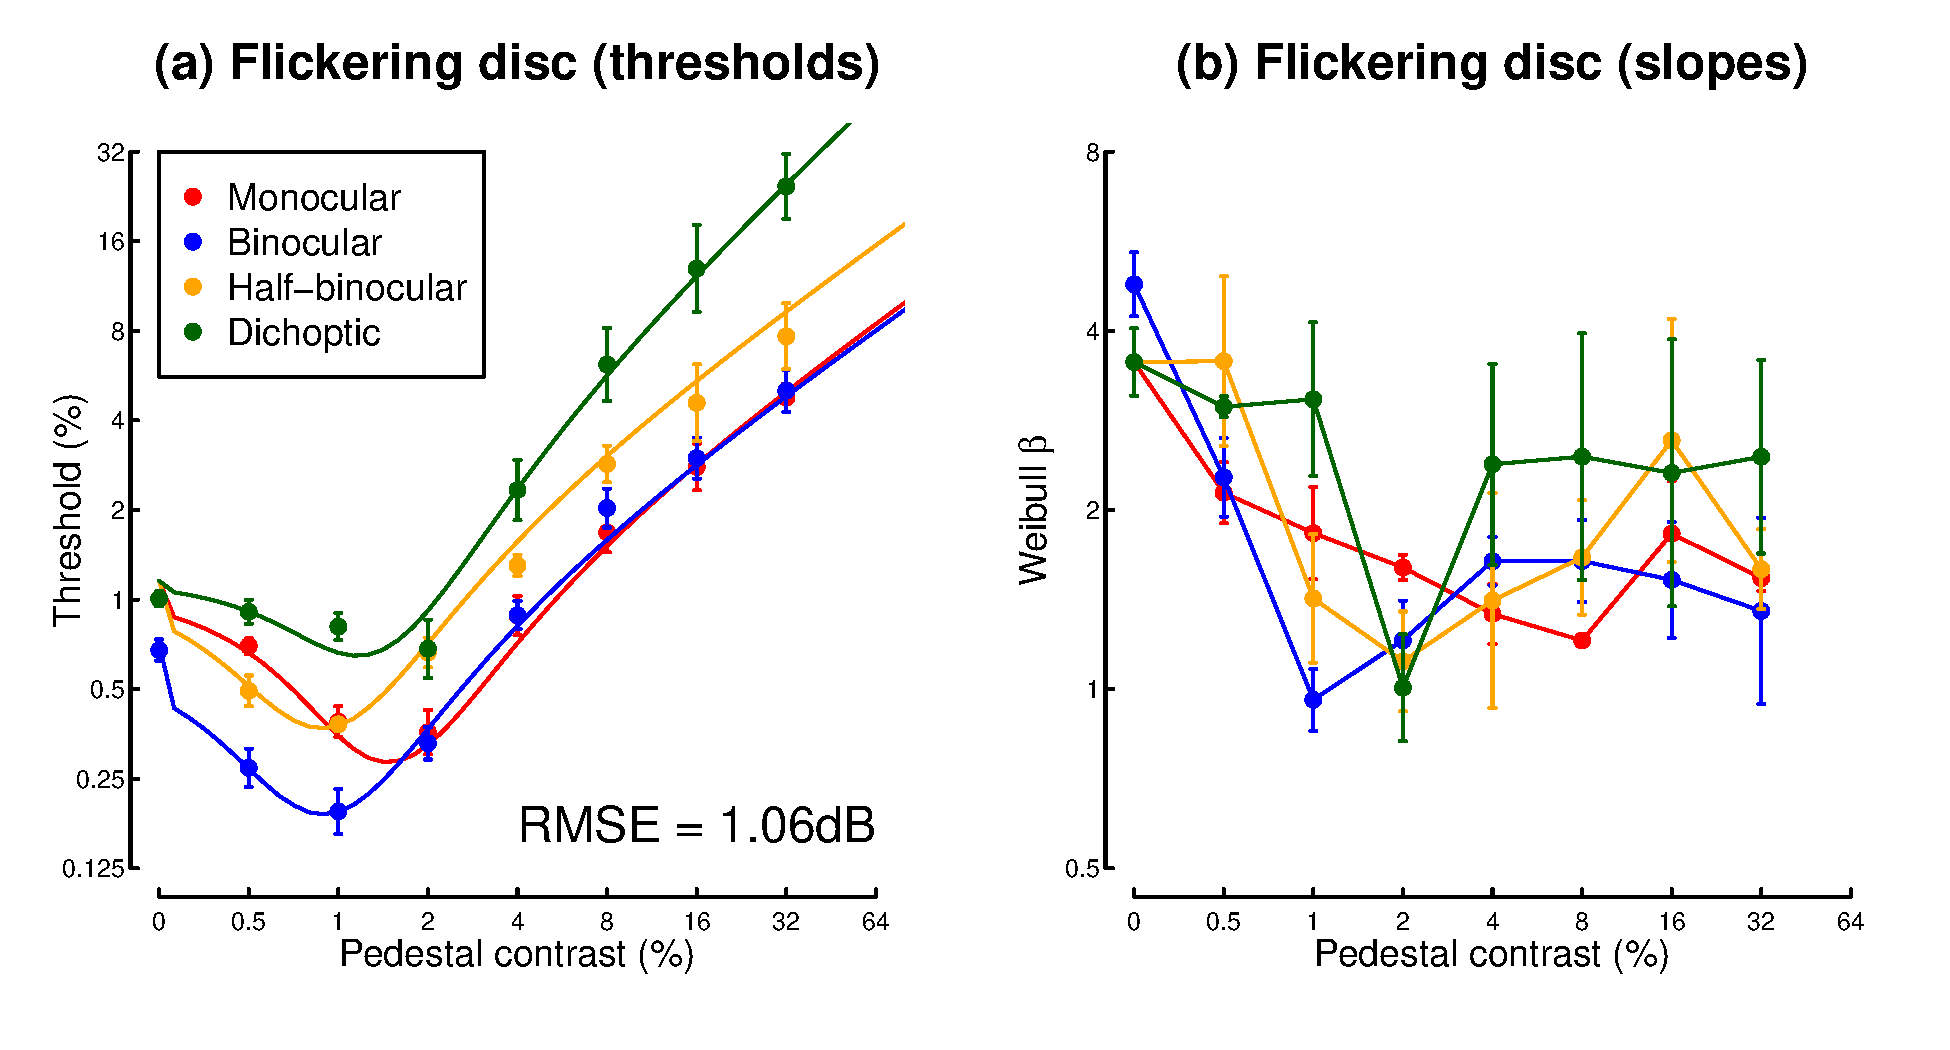
\includegraphics[width=0.8\textwidth,height=\textheight]{Figures/discdata.pdf}

}

\caption{\label{fig-discdata}Thresholds for the flickering disc
experiment. Plotting conventions mirror those in Figure 4.}

\end{figure}%

\subsection{Computational modelling}\label{computational-modelling}

\begin{table}

\caption{\label{tbl-parametertable}Summary of fitted model parameters.
The top row gives the best fitting parameters from the study of Meese et
al.~(2006). The second section shows the best fitting parameters from
simplex fits to the averaged thresholds for each experiment. The final
rows show the posterior parameter estimates from the Bayesian model,
fitted to each data set from Experiments 1 and 3.}

\centering{

\begin{tabular}[t]{lrrrrrrrr}
\toprule
\textbf{\em{Model fit}} & \textbf{\em{p}} & \textbf{\em{q}} & \textbf{\em{m}} & \textbf{\em{S}} & \textbf{\em{Z}} & \textbf{\em{$\omega$}} & \textbf{\em{k}} & \textbf{\em{RMSE}}\\
\midrule
Meese et al. (2006) & 7.99 & 6.59 & 1.28 & 0.99 & 0.08 & 1.00 & 0.19 & \\
\midrule
\textbf{Simplex fits} & \textbf{} & \textbf{} & \textbf{} & \textbf{} & \textbf{} & \textbf{} & \textbf{} & \textbf{}\\
Achromatic gratings & 5.96 & 4.69 & 1.34 & 0.87 & 0.13 & 1.00 & 0.20 & 1.59 dB\\
L-M gratings & 7.77 & 5.19 & 1.17 & 0.55 & 0.07 & 1.00 & 0.17 & 1.39 dB\\
S-(L+M) gratings & 16.01 & 11.56 & 1.13 & 0.33 & 0.00 & 0.99 & 0.27 & 1.46 dB\\
Flickering discs & 5.62 & 4.51 & 1.26 & 0.95 & 0.25 & 0.89 & 0.13 & 1.05 dB\\
\midrule
\textbf{Bayesian model} & \textbf{} & \textbf{} & \textbf{} & \textbf{} & \textbf{} & \textbf{} & \textbf{} & \textbf{}\\
Achromatic gratings & 7.06 & 5.63 & 1.27 & 0.63 & 0.08 & 0.98 & 0.30 & \\
L-M gratings & 5.11 & 3.63 & 1.24 & 1.22 & 0.03 & 1.05 & 0.19 & \\
S-(L+M) gratings & 6.78 & 5.34 & 1.24 & 0.61 & 0.01 & 0.95 & 0.34 & \\
Flickering discs & 7.16 & 5.76 & 1.25 & 0.65 & 0.13 & 0.87 & 0.24 & \\
\bottomrule
\end{tabular}

}

\end{table}%

For consistency with previous work, we initially performed least-squares
fits of the two-stage model (Meese et al., 2006) for each of the
chromaticity experiments, and the flickering disc experiment (7 free
parameters per fit). The best model fits are shown by the curves in
Figure~\ref{fig-dipperfig} and Figure~\ref{fig-discdata}, and provide an
excellent description of the data, with RMS errors between 1.05 and
1.59dB. Best fitting parameters are shown in the `Simplex fits' section
of Table~\ref{tbl-parametertable}. We note that in previous work, the
weight of interocular suppression (\(\omega\) in the model) was
implicitly fixed at 1. Here we allowed it to vary, but it still received
a value very close to 1 in all of our grating conditions, and slightly
below 1 (0.89) for our flickering discs. The exponent values (\emph{p}
and \emph{q}) for the S-(L+M) gratings are rather different from those
of the other conditions. In previous work (Meese et al., 2006) the
second stage gain control nonlinearity (Equation~\ref{eq-s2}) does
typically have quite substantial exponent values, which balance the
relatively mild nonlinearity at the first stage, and produce a
compressive transducer that results in contrast masking (the handle of
the dipper). The high value of \emph{p} = 16.01 is therefore likely to
be compensating for the low value of \emph{m} = 1.13 at stage one, but
may well represent the combination of several successive stages of
nonlinearity, and perhaps also other phenomena such as uncertainty
(Pelli, 1985).

We additionally implemented a hierarchical Bayesian version of the model
to estimate full posterior parameter distributions. This model was fit
simultaneously to the full trial-by-trial data from all participants who
completed a given experiment (i.e.~the model was fitted separately to
each of the four dipper data sets). Figure~\ref{fig-bayesianmodel}a-d
summarises the model behaviour, which displays the same pattern of
dipper functions as we found empirically. Modal posterior parameter
values (maximum a posteriori (MAP) estimates) are given in the lower
rows of Table~\ref{tbl-parametertable}. These are in a similar range to
the parameters from the simplex fitting and the original Meese et al.
(2006) parameters (reproduced in the first row of the table for
reference). The panels along the right and upper margins of
Figure~\ref{fig-bayesianmodel} show posterior distributions for each
model parameter. Note in particular that the posterior distribution for
the weight of interocular suppression (\(\omega\), top right panel)
overlaps 1 for each experiment, consistent with the strong dichoptic
masking observed in the threshold data. We note that the distribution
for \(\omega\) in the flickering disc condition is somewhat lower than
for the other three data sets. However this difference is not meaningful
according to widely accepted criteria such as comparing the 95\%
intervals of the distribution to a value of \(\omega=1\).

\begin{figure}

\centering{

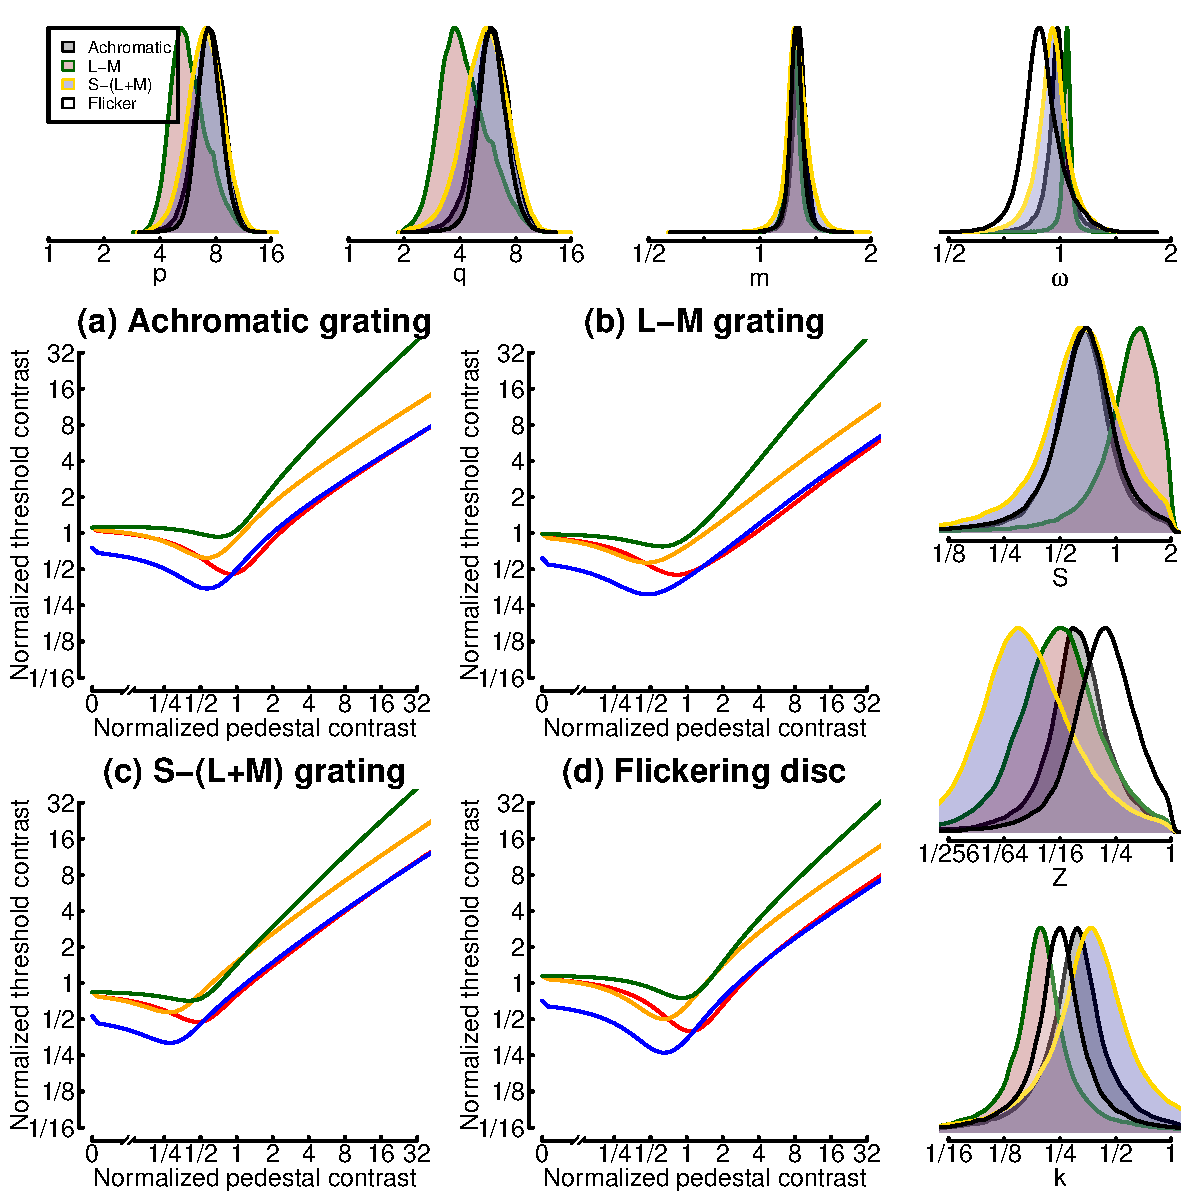
\includegraphics{Figures/stanoutput.pdf}

}

\caption{\label{fig-bayesianmodel}Model predictions (a-d) and posterior
parameters (top and right margin plots) for the hierarchical Bayesian
model. Curves in panels (a-d) show thresholds generated using the
maximum a posteriori parameter estimates. The probability density
functions in the margin plots are peak-normalized, and shown for each of
the four data sets in different colours (see legend in upper left plot).
Distributions were generated from 1000000 samples per data set, using a
Markov Chain Monte Carlo sampling algorithm. Note the logarithmic x-axis
for all posterior plots.}

\end{figure}%

Finally we fitted an extended model, that included interocular
suppression between the different pathways (see
Equation~\ref{eq-s1multi}), to the data of Experiment 2.
Figure~\ref{fig-MCSmodel} shows the model curves (panels a-c), which
correspond closely to the data in Figure~\ref{fig-MCSfig}. One striking
discrepancy is that the model predicts a region of negative d-prime for
the case where the target and dichoptic mask have the same chromaticity
(see the curved regions below 50\% correct). This happens in the model
because low contrast targets suppress the mask more than they excite the
detecting mechanism, producing a net decrease in response. The feature
(termed a `swan function') was not generally present in our empirical
data, though it can be observed for one participant in
Figure~\ref{fig-individualMCS}b,c.~Our previous work (Baker et al.,
2013) has found evidence for this phenomenon, but it generally requires
very high mask contrasts to be measurable empirically, and there may
also be some individual differences; both factors might explain its
absence here.

Figure~\ref{fig-MCSmodel}d,e shows the model estimates for the weight of
interocular suppression in each combination of target and mask
chromaticity. The weakest suppression was between achromatic targets and
masks and S-(L+M) targets and masks, and the strongest suppression was
between L-M targets and S-(L+M) masks. Note that the weight parameter
value of \(\omega\) = 1.11 for this condition is slightly higher than
that of the within-channel weights (values around 1), even though the
within-channel conditions generate more threshold elevation. In the
model, high thresholds for within-channel dichoptic masks occur because
the target and mask are summed together, which causes additional masking
(see Baker et al., 2013). However it is clear that the posterior
distribution of the weight parameter is quite broad and overlaps 1, so
this difference may not be meaningful. There do not appear to be any
other salient patterns in the suppressive weight estimates.

\begin{figure}

\centering{

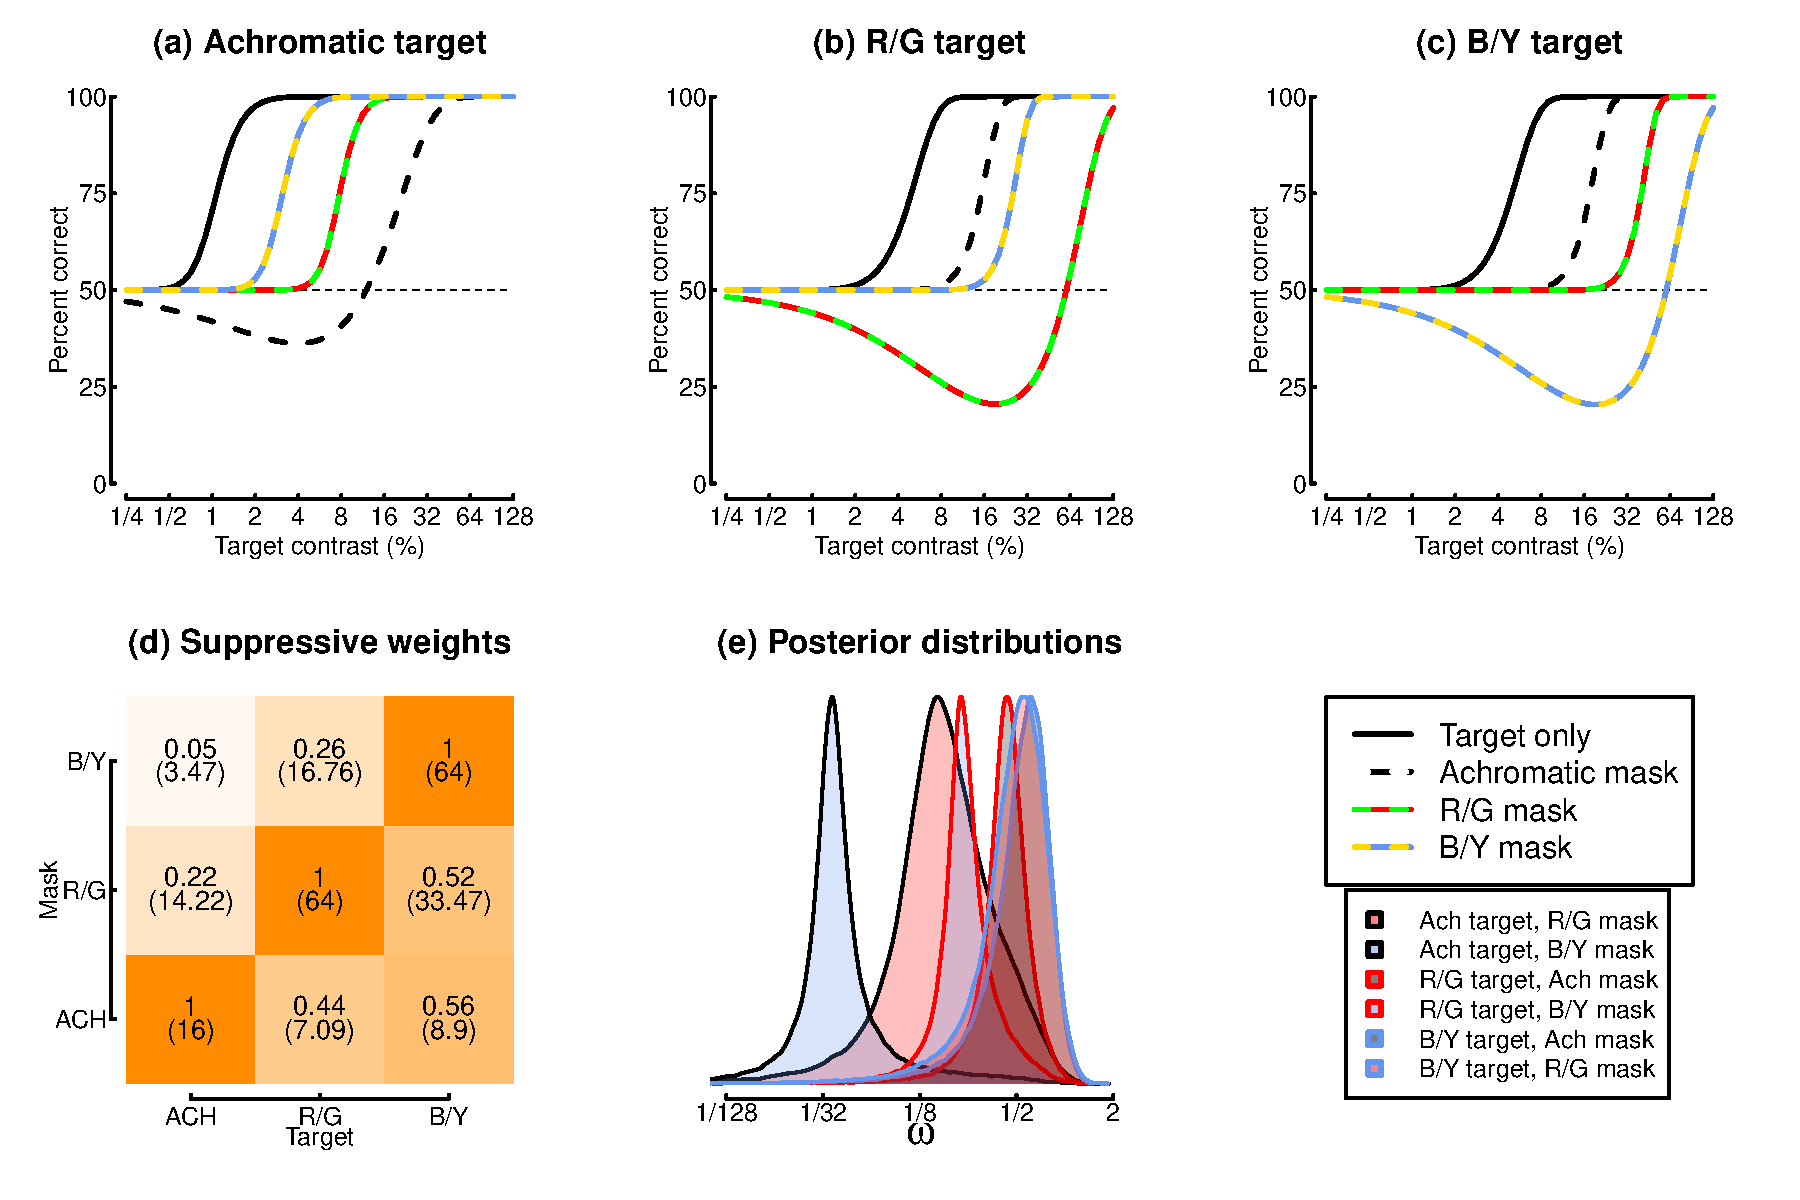
\includegraphics{Figures/MCSmodel.pdf}

}

\caption{\label{fig-MCSmodel}Summary of the model fit to the data of
Experiment 2. Panels (a-c) show model psychometric functions in the same
format as those in Figure 5. Panel (d) shows the fitted suppressive
weights (\(\omega\) values) estimated by the model, and panel (e) shows
the posterior distributions for each weight parameter. The lower right
plot gives the legends for the upper row (top) and the posterior
distributions in panel (e).}

\end{figure}%

\section{Discussion}\label{discussion}

Across three psychophysical experiments, we have demonstrated that:

\begin{itemize}
\tightlist
\item
  Binocular combination of isoluminant chromatic stimuli is similar to
  that for achromatic stimuli
\item
  Interocular suppression is strongest within a post-retinal pathway,
  and weakest between the achromatic and S-(L+M) pathways
\item
  Binocular combination occurs similarly for spatial and temporal
  luminance modulations
\end{itemize}

We now discuss the relationship to previous work, and consider the
likely physiological substrates of these effects.

\subsection{Summation at threshold}\label{summation-at-threshold}

Estimates of the binocular summation ratio at threshold fell within the
range \(\sqrt{2}\) to 2 for all four stimuli tested here. Consistent
with previous reports (Simmons, 2005), summation was slightly higher for
chromatic versus achromatic stimuli, but fell short of perfect linear
summation (a ratio of 2). In our model, summation at threshold is
determined by the exponent at the first gain control stage (the \emph{m}
parameter in Equation~\ref{eq-s1l} and Equation~\ref{eq-s1r}). The
summation ratio can be approximated by \(2^{1/m}\) (see Figure 9 of
Baker et al., 2012), such that an exponent of \(m=1\) produces a ratio
of 2, and an exponent of \(m = 2\) produces a ratio of \(\sqrt{2}\).
Both the simplex and Bayesian model fits (see
Table~\ref{tbl-parametertable}) generated parameter estimates in the
range \(1 < m < 1.4\), consistent with the high levels of summation
observed empirically. Note that the exponents at stage 2 (\(p\) and
\(q\)) have no effect on binocular summation at threshold, because they
impact after the signals have been combined. The differences in these
parameter values between chromatic conditions (see
Table~\ref{tbl-parametertable}) primarily reflects differences in the
slope of the dipper handle (chromatic conditions are shallower), and are
of incidental interest for our main questions.

\subsection{Interocular suppression}\label{interocular-suppression}

The weight of interocular suppression is represented by the model
parameter, \(\omega\) (Equation~\ref{eq-s1l} and Equation~\ref{eq-s1r}).
Posterior distributions of this parameter overlapped 1 for all of our
dipper function data sets (see top right panel in
Figure~\ref{fig-bayesianmodel}), indicating strong interocular
suppression regardless of post-retinal pathway. The flickering disc
stimuli produced a slightly lower suppression estimate, with
\(\omega < 0.9\). This may indicate slightly weaker suppression between
the eyes for temporal modulations, but it is much less extreme than our
recent estimates using EEG and matching paradigms (Segala et al., 2023).
One difference between these studies is the luminance of the background,
which was set to black for the experiments of Segala et al. (2023), but
here was set at the mean luminance. Other studies using static luminance
increments have also reported differences in the character of binocular
combination that are attributable to background luminance (Baker et al.,
2012), so this may explain the differences between studies. We also note
that the weaker interocular suppression for flickering disc stimuli
appears to be largely due to one participant (see
Figure~\ref{fig-individualdiscs}c), so individual differences might also
play a role. Future work should manipulate the background luminance
systematically to better understand how this modulates interocular
suppression.

Strong interocular suppression is responsible for the convergence of
monocular and binocular dipper handles (e.g. Legge, 1984) at high
pedestal contrasts (see Figure~\ref{fig-dipperfig}). In the model,
monocular stimuli avoid the impact of interocular suppression, because
the unstimulated eye sees a blank screen, and so contributes a contrast
of zero to the denominator of the stimulated eye. Binocular stimuli
receive strong suppression, which acts to approximately halve the
excitation when contrasts in the two eyes are equal (see Georgeson et
al., 2016; Meese et al., 2006). This normalization leads to very similar
responses for monocular and binocular stimulation. In the auditory
system, binaural combination of amplitude modulated signals involves
much weaker suppression between channels, and the monaural and binaural
dipper handles do not converge at high contrasts (Baker et al., 2020).

One phenomenon that often occurs with conflicting dichoptic stimuli is
binocular rivalry, and it is worth considering how this might impact the
results of Experiment 2, where the two eyes often saw stimuli of
different chromaticities. However rivalry typically only `kicks in' at
presentation durations longer than the 200ms used here (see e.g. Wolfe,
1983), and certainly rivalry alternations need much longer presentations
to be clearly observed. In a dichoptic masking paradigm it is often
difficult to distinguish dichoptic fusion from dominance of one eye over
the other; indeed, interocular suppression of sufficient strength would
render the weaker stimulus invisible. On the other hand, if the stimuli
appear fused, we might expect dichoptic colour mixing to occur (Kingdom
\& Libenson, 2015; Kingdom \& Wang, 2015), whereas if one eye dominates
the colour percept would be equivalent to monocular presentation of the
dominant stimulus. Here we used a performance task (2AFC
detection/discrimination), and did not explicitly ask participants about
the stimulus appearance. Future studies could use matching and
adjustment tasks to investigate this further.

\subsection{Psychometric slopes}\label{psychometric-slopes}

Previous work has demonstrated that the slope of the psychometric
function in 2AFC tasks can distinguish different types of masking,
although it is much less widely reported than threshold measures. In
particular, pedestal masking linearizes the slope (Foley \& Legge, 1981;
Meese et al., 2006), and within-channel dichoptic masking produces very
steep slopes (Baker et al., 2013; Meese et al., 2006). We replicate both
of these effects here, and show that they extend to the isoluminant
chromatic pathways (see Figure~\ref{fig-dipperfig}d-f \&
Figure~\ref{fig-MCSfig}). We additionally show that dichoptic masking
between different pathways does not produce unusually steep slopes (see
Figure~\ref{fig-MCSfig}). It therefore more closely resembles other
types of masking between visual channels, such as cross-orientation
masking (Meese \& Baker, 2009), surround masking (Yu et al., 2002), and
masking from broadband noise (Baker \& Meese, 2012; Lu \& Dosher, 2008),
which also do not impact psychometric slopes.

\subsection{Physiological substrates}\label{physiological-substrates}

Recent evidence indicates that the physiological substrate of
interocular suppression may be neurons in layer 4 of primary visual
cortex (Dougherty et al., 2019). Most cells in this layer are
monocularly excitable, in that their responses increase only by
stimulation of their preferred eye. However, simultaneous stimulation of
the non-preferred eye can modulate the response, usually in an
inhibitory fashion, exactly as proposed at stage 1 of the two-stage
model (Equation~\ref{eq-s1l} and Equation~\ref{eq-s1r}). In terms of
perception, one consequence of this early suppression is to achieve
`ocularity invariance', whereby the perceived contrast of a stimulus
viewed by one eye is equivalent to that of the same stimulus viewed by
both eyes (Baker et al., 2007). Similar processes of response invariance
have also been reported using fMRI (Moradi \& Heeger, 2009) and
steady-state EEG (Baker \& Wade, 2017).

In V1, the classical view was that chromatic stimuli are processed in
`blob' regions that are largely monocular as they fall within ocular
dominance columns (Livingstone \& Hubel, 1984). However more recent work
has shown chromatic processing outside of the blobs (Sincich \& Horton,
2005), especially for stimuli with spatial structure (Chatterjee et al.,
2021). Since our psychophysical results indicate that interocular
suppression is equally strong within chromatic and achromatic pathways,
it may be that psychophysical performance indexes a common population of
(non-blob) neurons for all of our stimuli. On the other hand, if blob
regions include a subset of monocular neurons subject to interocular
suppression (e.g. Dougherty et al., 2019), this might be followed by
binocular summation at a later stage of processing for chromatic
stimuli, and potentially also for very low spatial frequency luminance
modulations also processed in blobs (Economides et al., 2011).

\section{Conclusions}\label{conclusions}

Here we provide estimates of interocular suppression within and between
the three primary post-retinal visual pathways. These results show that
binocular signal combination is similar within each pathway, but that
interocular suppression is typically weaker between pathways. Our
findings could be applied when building models to predict perception of
binocular images and movies, for example those generated by virtual and
augmented reality systems, or in 3D cinema and television.

\section{Acknowledgements}\label{acknowledgements}

Supported by BBSRC grant BB/V007580/1 awarded to DHB and ARW.

\section{References}\label{references}

\phantomsection\label{refs}
\begin{CSLReferences}{1}{0}
\bibitem[\citeproctext]{ref-Anstis1998}
Anstis, S., \& Ho, A. (1998). Nonlinear combination of luminance
excursions during flicker, simultaneous contrast, afterimages and
binocular fusion. \emph{Vision Res}, \emph{38}(4), 523--539.
\url{https://doi.org/10.1016/s0042-6989(97)00167-3}

\bibitem[\citeproctext]{ref-Baker2018}
Baker, D. H., Lygo, F. A., Meese, T. S., \& Georgeson, M. A. (2018).
Binocular summation revisited: Beyond \(\sqrt{2}\). \emph{Psychol Bull},
\emph{144}(11), 1186--1199. \url{https://doi.org/10.1037/bul0000163}

\bibitem[\citeproctext]{ref-Baker2007b}
Baker, D. H., \& Meese, T. S. (2007). Binocular contrast interactions:
Dichoptic masking is not a single process. \emph{Vision Res},
\emph{47}(24), 3096--3107.
\url{https://doi.org/10.1016/j.visres.2007.08.013}

\bibitem[\citeproctext]{ref-Baker2012b}
Baker, D. H., \& Meese, T. S. (2012). Zero-dimensional noise: The best
mask you never saw. \emph{J Vis}, \emph{12}(10).
\url{https://doi.org/10.1167/12.10.20}

\bibitem[\citeproctext]{ref-Baker2007}
Baker, D. H., Meese, T. S., \& Georgeson, M. A. (2007). Binocular
interaction: Contrast matching and contrast discrimination are predicted
by the same model. \emph{Spat Vis}, \emph{20}(5), 397--413.
\url{https://doi.org/10.1163/156856807781503622}

\bibitem[\citeproctext]{ref-Baker2013}
Baker, D. H., Meese, T. S., \& Georgeson, M. A. (2013). Paradoxical
psychometric functions ("swan functions") are explained by dilution
masking in four stimulus dimensions. \emph{{iPerception}}, \emph{4}(1),
17--35. \url{https://doi.org/10.1068/i0552}

\bibitem[\citeproctext]{ref-Baker2020}
Baker, D. H., Vilidaite, G., McClarnon, E., Valkova, E., Bruno, A., \&
Millman, R. E. (2020). Binaural summation of amplitude modulation
involves weak interaural suppression. \emph{Sci Rep}, \emph{10}(1),
3560. \url{https://doi.org/10.1038/s41598-020-60602-5}

\bibitem[\citeproctext]{ref-Baker2017}
Baker, D. H., \& Wade, A. R. (2017). Evidence for an optimal algorithm
underlying signal combination in human visual cortex. \emph{Cereb
Cortex}, \emph{27}(1), 254--264.
\url{https://doi.org/10.1093/cercor/bhw395}

\bibitem[\citeproctext]{ref-Baker2012}
Baker, D. H., Wallis, S. A., Georgeson, M. A., \& Meese, T. S. (2012).
Nonlinearities in the binocular combination of luminance and contrast.
\emph{Vision Res}, \emph{56}, 1--9.
\url{https://doi.org/10.1016/j.visres.2012.01.008}

\bibitem[\citeproctext]{ref-Campbell1965}
Campbell, F. W., \& Green, D. G. (1965). Monocular versus binocular
visual acuity. \emph{Nature}, \emph{208}(5006), 191--192.
\url{https://doi.org/10.1038/208191a0}

\bibitem[\citeproctext]{ref-Carpenter2017}
Carpenter, B., Gelman, A., Hoffman, M. D., Lee, D., Goodrich, B.,
Betancourt, M., Brubaker, M., Guo, J., Li, P., \& Riddell, A. (2017).
Stan: A probabilistic programming language. \emph{Journal of Statistical
Software}, \emph{76}(1), 1--32.
\url{https://doi.org/10.18637/jss.v076.i01}

\bibitem[\citeproctext]{ref-Chatterjee2021}
Chatterjee, S., Ohki, K., \& Reid, R. C. (2021). Chromatic micromaps in
primary visual cortex. \emph{Nat Commun}, \emph{12}(1), 2315.
\url{https://doi.org/10.1038/s41467-021-22488-3}

\bibitem[\citeproctext]{ref-Chen2000}
Chen, C., Foley, J. M., \& Brainard, D. H. (2000). Detection of
chromoluminance patterns on chromoluminance pedestals i: Threshold
measurements. \emph{Vision Res}, \emph{40}(7), 773--788.
\url{https://doi.org/10.1016/s0042-6989(99)00227-8}

\bibitem[\citeproctext]{ref-Cole1993}
Cole, G. R., Hine, T., \& McIlhagga, W. (1993). Detection mechanisms in
l-, m-, and s-cone contrast space. \emph{J Opt Soc Am A}, \emph{10}(1),
38--51. \url{https://doi.org/10.1364/josaa.10.000038}

\bibitem[\citeproctext]{ref-Cole1990}
Cole, G. R., Stromeyer, C. F., 3rd, \& Kronauer, R. E. (1990). Visual
interactions with luminance and chromatic stimuli. \emph{J Opt Soc Am
A}, \emph{7}(1), 128--140. \url{https://doi.org/10.1364/josaa.7.000128}

\bibitem[\citeproctext]{ref-Dougherty2019}
Dougherty, K., Cox, M. A., Westerberg, J. A., \& Maier, A. (2019).
Binocular modulation of monocular V1 neurons. \emph{Curr Biol},
\emph{29}(3), 381--391.e4.
\url{https://doi.org/10.1016/j.cub.2018.12.004}

\bibitem[\citeproctext]{ref-Economides2011}
Economides, J. R., Sincich, L. C., Adams, D. L., \& Horton, J. C.
(2011). Orientation tuning of cytochrome oxidase patches in macaque
primary visual cortex. \emph{Nat Neurosci}, \emph{14}(12), 1574--1580.
\url{https://doi.org/10.1038/nn.2958}

\bibitem[\citeproctext]{ref-Ernst2002}
Ernst, M. O., \& Banks, M. S. (2002). Humans integrate visual and haptic
information in a statistically optimal fashion. \emph{Nature},
\emph{415}(6870), 429--433. \url{https://doi.org/10.1038/415429a}

\bibitem[\citeproctext]{ref-Foley1981}
Foley, J. M., \& Legge, G. E. (1981). Contrast detection and
near-threshold discrimination in human vision. \emph{Vision Res},
\emph{21}(7), 1041--1053.
\url{https://doi.org/10.1016/0042-6989(81)90009-2}

\bibitem[\citeproctext]{ref-Georgeson2016}
Georgeson, M. A., Wallis, S. A., Meese, T. S., \& Baker, D. H. (2016).
Contrast and lustre: A model that accounts for eleven different forms of
contrast discrimination in binocular vision. \emph{Vision Res},
\emph{129}, 98--118. \url{https://doi.org/10.1016/j.visres.2016.08.001}

\bibitem[\citeproctext]{ref-Horton1981}
Horton, J. C., \& Hubel, D. H. (1981). Regular patchy distribution of
cytochrome oxidase staining in primary visual cortex of macaque monkey.
\emph{Nature}, \emph{292}(5825), 762--764.
\url{https://doi.org/10.1038/292762a0}

\bibitem[\citeproctext]{ref-Kim2013}
Kim, Y. J., Gheiratmand, M., \& Mullen, K. T. (2013). Cross-orientation
masking in human color vision: Application of a two-stage model to
assess dichoptic and monocular sources of suppression. \emph{J Vis},
\emph{13}(6), 15. \url{https://doi.org/10.1167/13.6.15}

\bibitem[\citeproctext]{ref-Kim2015}
Kim, Y. J., \& Mullen, K. T. (2015). The dynamics of cross-orientation
masking at monocular and interocular sites. \emph{Vision Res},
\emph{116}(Pt A), 80--91.
\url{https://doi.org/10.1016/j.visres.2015.09.008}

\bibitem[\citeproctext]{ref-Kingdom2015}
Kingdom, F. A. A., \& Libenson, L. (2015). Dichoptic color saturation
mixture: Binocular luminance contrast promotes perceptual averaging.
\emph{J Vis}, \emph{15}(5), 2. \url{https://doi.org/10.1167/15.5.2}

\bibitem[\citeproctext]{ref-Kingdom2015b}
Kingdom, F. A. A., \& Wang, D. (2015). Dichoptic colour-saturation
masking is unmasked by binocular luminance contrast. \emph{Vision Res},
\emph{116}(Pt A), 45--52.
\url{https://doi.org/10.1016/j.visres.2015.08.016}

\bibitem[\citeproctext]{ref-Legge1979}
Legge, G. E. (1979). Spatial frequency masking in human vision:
Binocular interactions. \emph{J Opt Soc Am}, \emph{69}(6), 838--847.
\url{https://doi.org/10.1364/josa.69.000838}

\bibitem[\citeproctext]{ref-Legge1984}
Legge, G. E. (1984). Binocular contrast summation--II. Quadratic
summation. \emph{Vision Res}, \emph{24}(4), 385--394.
\url{https://doi.org/10.1016/0042-6989(84)90064-6}

\bibitem[\citeproctext]{ref-Levelt1965}
Levelt, W. J. (1965). Binocular brightness averaging and contour
information. \emph{Br J Psychol}, \emph{56}, 1--13.
\url{https://doi.org/10.1111/j.2044-8295.1965.tb00939.x}

\bibitem[\citeproctext]{ref-Livingstone1984}
Livingstone, M. S., \& Hubel, D. H. (1984). Anatomy and physiology of a
color system in the primate visual cortex. \emph{J Neurosci},
\emph{4}(1), 309--356.
\url{https://doi.org/10.1523/JNEUROSCI.04-01-00309.1984}

\bibitem[\citeproctext]{ref-Lu2008}
Lu, Z.-L., \& Dosher, B. A. (2008). Characterizing observers using
external noise and observer models: Assessing internal representations
with external noise. \emph{Psychol Rev}, \emph{115}(1), 44--82.
\url{https://doi.org/10.1037/0033-295X.115.1.44}

\bibitem[\citeproctext]{ref-Maehara2005}
Maehara, G., \& Goryo, K. (2005). Binocular, monocular and dichoptic
pattern masking. \emph{Optical Review}, \emph{12}(2), 76--82.
\url{https://doi.org/10.1007/PL00021542}

\bibitem[\citeproctext]{ref-Medina2009}
Medina, J. M., \& Mullen, K. T. (2009). Cross-orientation masking in
human color vision. \emph{J Vis}, \emph{9}(3), 20.1--16.
\url{https://doi.org/10.1167/9.3.20}

\bibitem[\citeproctext]{ref-Meese2009}
Meese, T. S., \& Baker, D. H. (2009). Cross-orientation masking is speed
invariant between ocular pathways but speed dependent within them.
\emph{J Vis}, \emph{9}(5), 2.1--15. \url{https://doi.org/10.1167/9.5.2}

\bibitem[\citeproctext]{ref-Meese2006}
Meese, T. S., Georgeson, M. A., \& Baker, D. H. (2006). Binocular
contrast vision at and above threshold. \emph{J Vis}, \emph{6}(11),
1224--1243. \url{https://doi.org/10.1167/6.11.7}

\bibitem[\citeproctext]{ref-Moradi2009}
Moradi, F., \& Heeger, D. J. (2009). Inter-ocular contrast normalization
in human visual cortex. \emph{J Vis}, \emph{9}(3), 13.1--22.
\url{https://doi.org/10.1167/9.3.13}

\bibitem[\citeproctext]{ref-Mullen2014}
Mullen, K. T., Kim, Y. J., \& Gheiratmand, M. (2014). Contrast
normalization in colour vision: The effect of luminance contrast on
colour contrast detection. \emph{Sci Rep}, \emph{4}, 7350.
\url{https://doi.org/10.1038/srep07350}

\bibitem[\citeproctext]{ref-Mullen1994}
Mullen, K. T., \& Losada, M. A. (1994). Evidence for separate pathways
for color and luminance detection mechanisms. \emph{J Opt Soc Am A Opt
Image Sci Vis}, \emph{11}(12), 3136--3151.
\url{https://doi.org/10.1364/josaa.11.003136}

\bibitem[\citeproctext]{ref-Pelli1985}
Pelli, D. G. (1985). Uncertainty explains many aspects of visual
contrast detection and discrimination. \emph{J Opt Soc Am A},
\emph{2}(9), 1508--1532. \url{https://doi.org/10.1364/josaa.2.001508}

\bibitem[\citeproctext]{ref-Read2021}
Read, J. C. A. (2021). Binocular vision and stereopsis across the animal
kingdom. \emph{Annu Rev Vis Sci}, \emph{7}, 389--415.
\url{https://doi.org/10.1146/annurev-vision-093019-113212}

\bibitem[\citeproctext]{ref-Schutt2016}
Schütt, H. H., Harmeling, S., Macke, J. H., \& Wichmann, F. A. (2016).
Painfree and accurate bayesian estimation of psychometric functions for
(potentially) overdispersed data. \emph{Vision Res}, \emph{122},
105--123. \url{https://doi.org/10.1016/j.visres.2016.02.002}

\bibitem[\citeproctext]{ref-Segala2023}
Segala, F. G., Bruno, A., Martin, J. T., Aung, M. T., Wade, A. R., \&
Baker, D. H. (2023). Different rules for binocular combination of
luminance flicker in cortical and subcortical pathways. \emph{eLife},
\emph{12}, RP87048. \url{https://doi.org/10.7554/eLife.87048}

\bibitem[\citeproctext]{ref-Shapley2011}
Shapley, R., \& Hawken, M. J. (2011). Color in the cortex: Single- and
double-opponent cells. \emph{Vision Res}, \emph{51}(7), 701--717.
\url{https://doi.org/10.1016/j.visres.2011.02.012}

\bibitem[\citeproctext]{ref-Sharpe2011}
Sharpe, L. T., Stockman, A., Jagla, W., \& Jägle, H. (2011). A luminous
efficiency function, VD65* (λ), for daylight adaptation: A correction.
\emph{Color Research \& Application}, \emph{36}(1), 42--46.
https://doi.org/\url{https://doi.org/10.1002/col.20602}

\bibitem[\citeproctext]{ref-Shooner2020}
Shooner, C., \& Mullen, K. T. (2020). Enhanced luminance sensitivity on
color and luminance pedestals: Threshold measurements and a model of
parvocellular luminance processing. \emph{J Vis}, \emph{20}(6), 12.
\url{https://doi.org/10.1167/jov.20.6.12}

\bibitem[\citeproctext]{ref-Simmons2005}
Simmons, D. R. (2005). The binocular combination of chromatic contrast.
\emph{Perception}, \emph{34}(8), 1035--1042.
\url{https://doi.org/10.1068/p5279}

\bibitem[\citeproctext]{ref-Sincich2005}
Sincich, L. C., \& Horton, J. C. (2005). The circuitry of V1 and V2:
Integration of color, form, and motion. \emph{Annu Rev Neurosci},
\emph{28}, 303--326.
\url{https://doi.org/10.1146/annurev.neuro.28.061604.135731}

\bibitem[\citeproctext]{ref-Stockman2000}
Stockman, A., \& Sharpe, L. T. (2000). The spectral sensitivities of the
middle- and long-wavelength-sensitive cones derived from measurements in
observers of known genotype. \emph{Vision Res}, \emph{40}(13),
1711--1737. \url{https://doi.org/10.1016/s0042-6989(00)00021-3}

\bibitem[\citeproctext]{ref-Switkes1988}
Switkes, E., Bradley, A., \& De Valois, K. K. (1988). Contrast
dependence and mechanisms of masking interactions among chromatic and
luminance gratings. \emph{J Opt Soc Am A}, \emph{5}(7), 1149--1162.
\url{https://doi.org/10.1364/josaa.5.001149}

\bibitem[\citeproctext]{ref-Wallis2013}
Wallis, S. A., Baker, D. H., Meese, T. S., \& Georgeson, M. A. (2013).
The slope of the psychometric function and non-stationarity of
thresholds in spatiotemporal contrast vision. \emph{Vision Res},
\emph{76}, 1--10. \url{https://doi.org/10.1016/j.visres.2012.09.019}

\bibitem[\citeproctext]{ref-Wolfe1983}
Wolfe, J. M. (1983). Influence of spatial frequency, luminance, and
duration on binocular rivalry and abnormal fusion of briefly presented
dichoptic stimuli. \emph{Perception}, \emph{12}(4), 447--456.
\url{https://doi.org/10.1068/p120447}

\bibitem[\citeproctext]{ref-Yu2002}
Yu, C., Klein, S. A., \& Levi, D. M. (2002). Facilitation of contrast
detection by cross-oriented surround stimuli and its psychophysical
mechanisms. \emph{J Vis}, \emph{2}(3), 243--255.
\url{https://doi.org/10.1167/2.3.4}

\end{CSLReferences}

\section{Appendices}\label{appendices}

\beginsupplement

\begin{figure}

\centering{

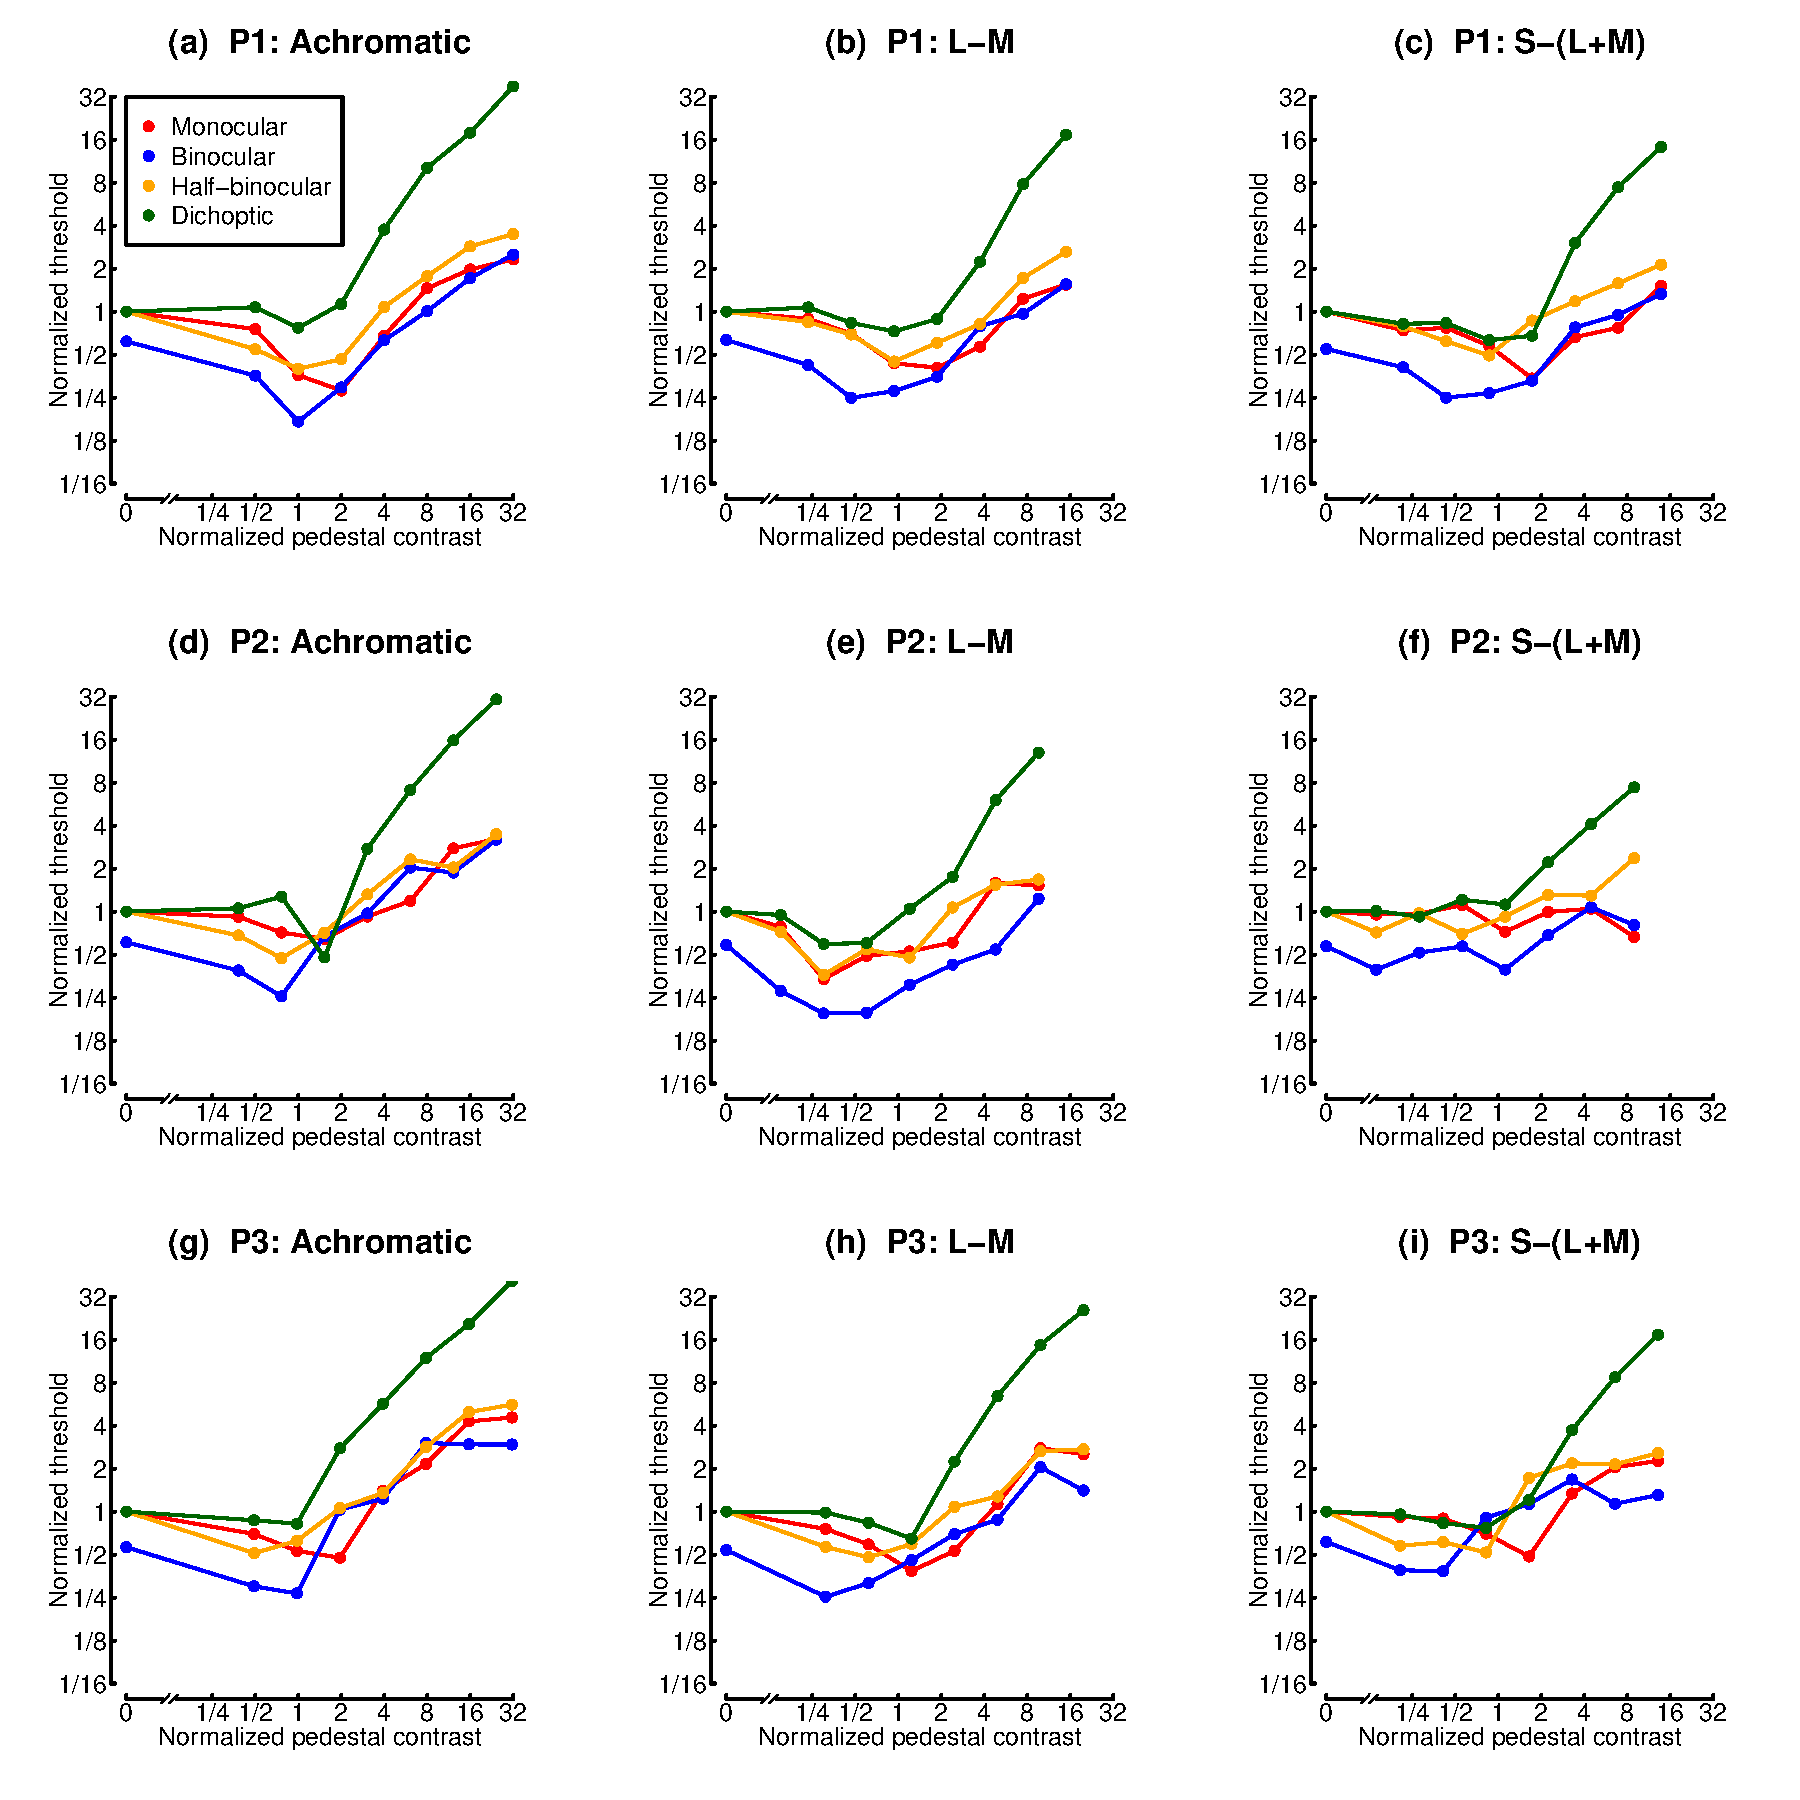
\includegraphics{Figures/individualdippers.pdf}

}

\caption{\label{fig-individualdippers}Individual participant data from
Experiment 1.}

\end{figure}%

\begin{figure}

\centering{

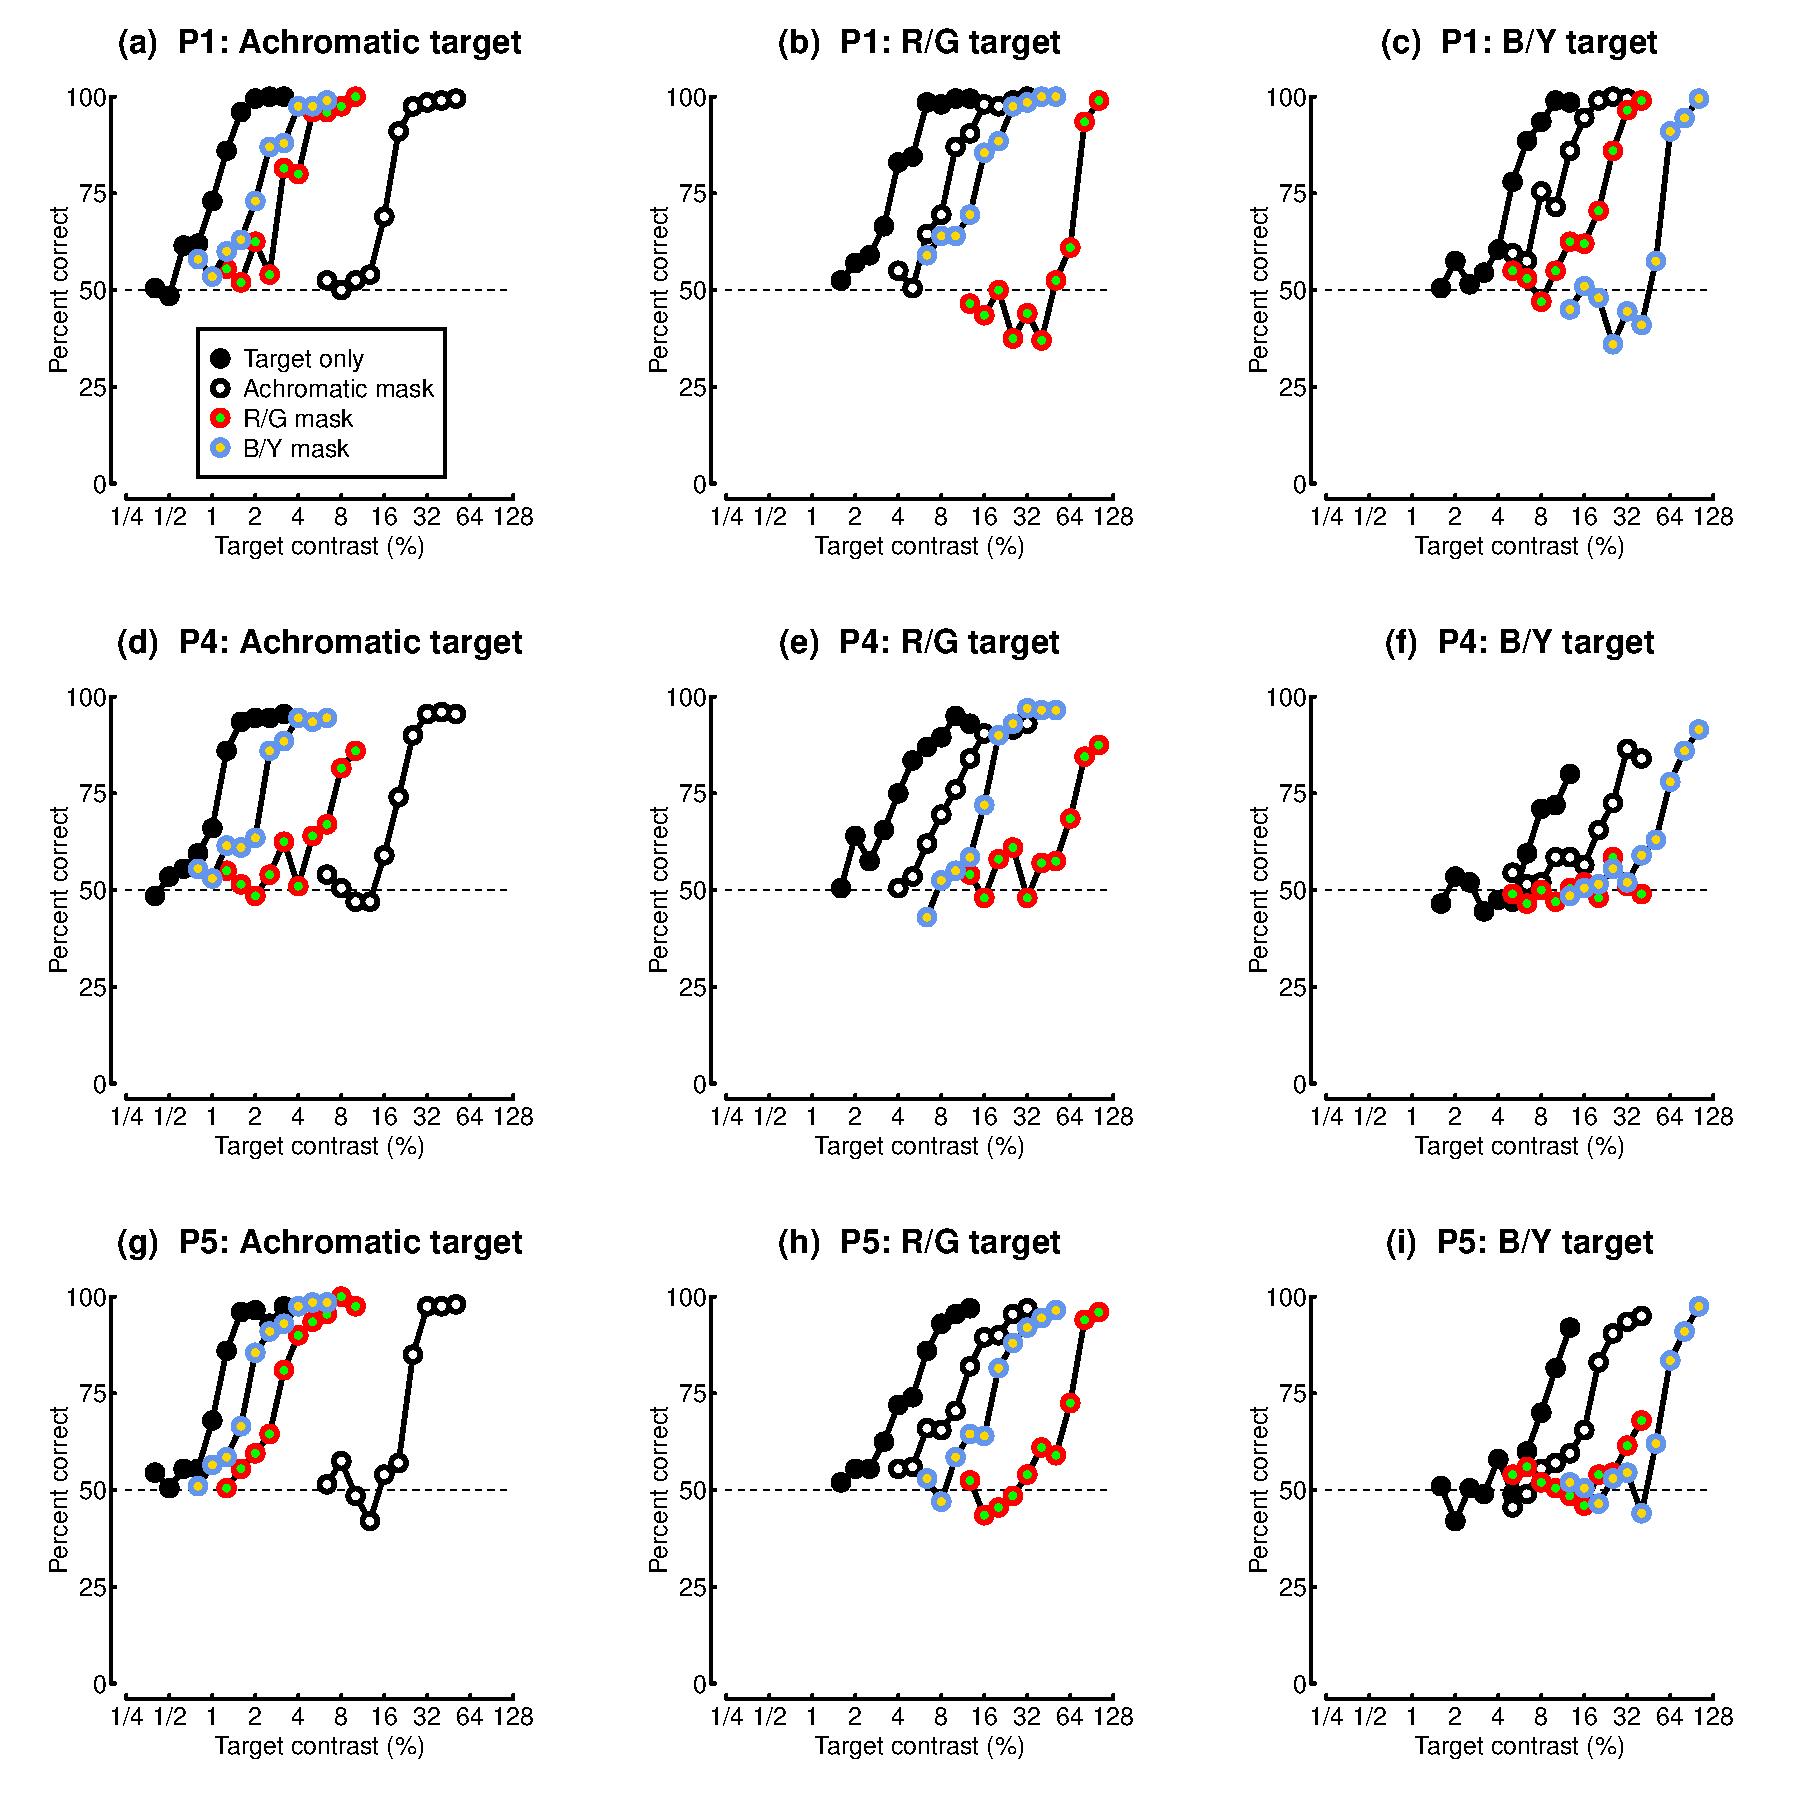
\includegraphics{Figures/individualMCS.pdf}

}

\caption{\label{fig-individualMCS}Individual participant data from
Experiment 2.}

\end{figure}%

\begin{figure}

\centering{

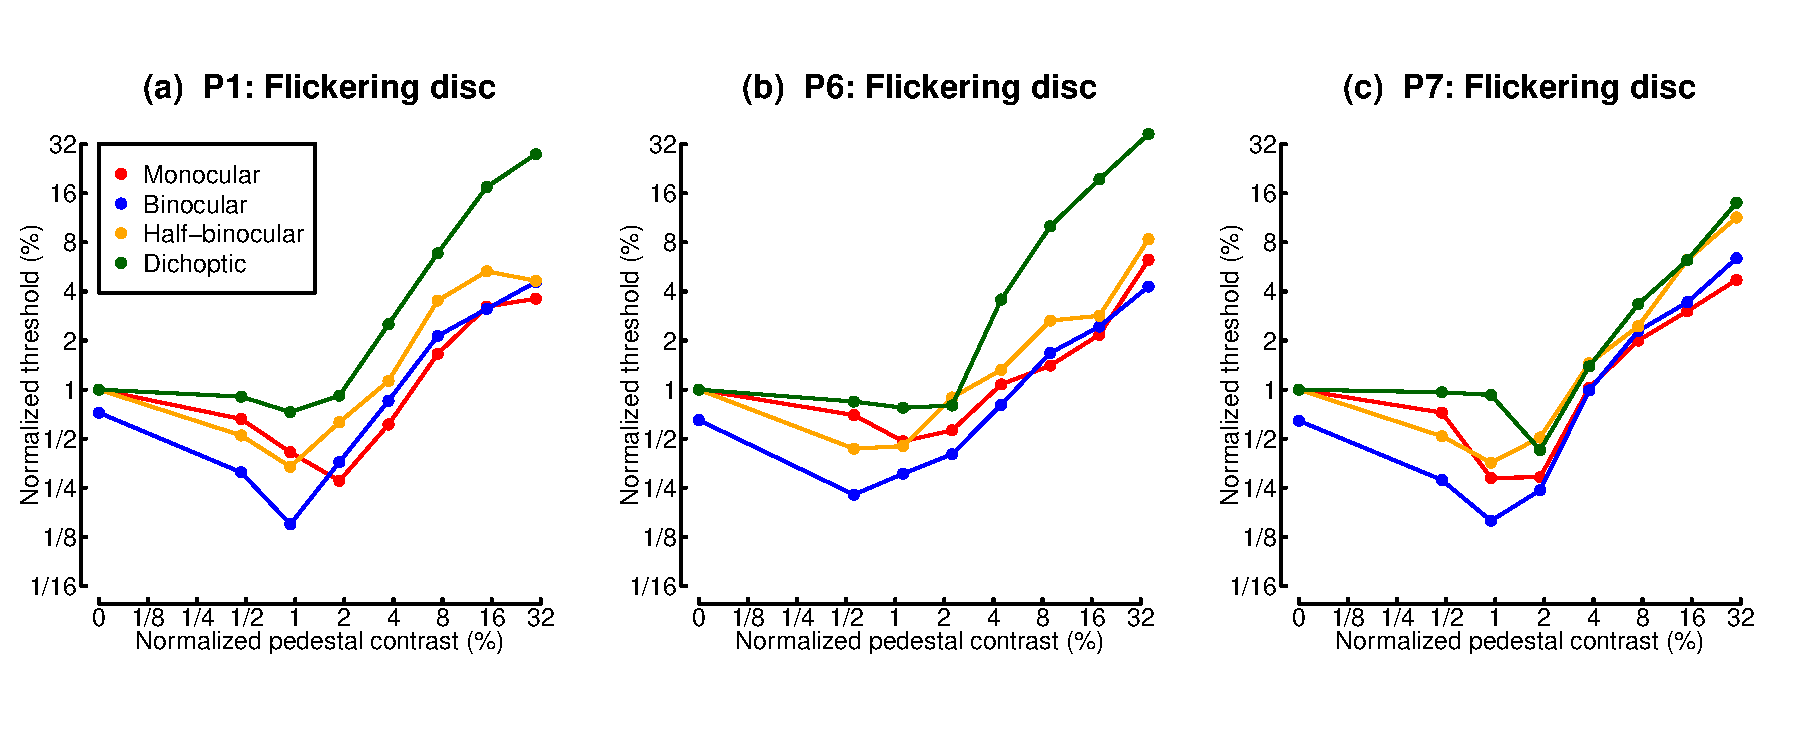
\includegraphics{Figures/individualdiscs.pdf}

}

\caption{\label{fig-individualdiscs}Individual participant data from
Experiment 3.}

\end{figure}%



\end{document}
